% Version 1.2.0 DE
%
%%%%%%%%%%%%%%%%%%%%%%%%%%%%%%%%%%%%%%%%%%%%%%%%%%
%%%        			Päambel!  				             %%%
%%%%%%%%%%%%%%%%%%%%%%%%%%%%%%%%%%%%%%%%%%%%%%%%%%

%%%%%%%%%%%%%%%%%%%%%%%%%%%%%%%%%%%%%%%%%%%%%%%%%%
%%%        			Päambel / Kompilieren!         %%%
%%%%%%%%%%%%%%%%%%%%%%%%%%%%%%%%%%%%%%%%%%%%%%%%%%

% Wichtig:
% Um Fehler und Probleme beim Kompilieren zu vermeiden, benutzen Sie bitte immer die aktuelle Version Ihres Betriebssystems (Windows / Mac / Linux), die aktuelle Version Ihrer LaTeX-Distribution (MiKTeX / MacTeX / Tex Live) und die aktuelle Version Ihres Setzprogramms beziehungsweise LaTeX-Editors (TeXstudio / Texmaker / TeXworks / TeXnicCenter). Aktualisieren Sie Ihr Betriebssystem, Ihre LaTeX-Distribution und Ihren LaTeX-Editor vor dem Kompilieren dieser Vorlage oder lassen Sie diese von Ihrem IT-Beauftragten der Abteilung aktualisieren.
%
% Hinweise zum Kompilieren / Setzreihenfolge:
% Für die korrekte Darstellung des Layouts sowie der Bibliografien (multibib) kompilieren Sie bitte wie folgt (siehe Reihenfolge der Kompiliervorgänge):
%
%- Windows 10: über die Eingabeaufforderung PowerShell bzw. Eingabeaufforderung (cmd).
% Gehen Sie dazu in den Ordner dieses Projekts, wählen Sie keine Datei an, klicken Sie auf eine leere Stelle mit der linken Maustaste und öffnen Sie das Kontextmenü bei gedrückter Umschalttaste (Umschalttaste + rechter Mausklick) und wählen Sie "PowerShell-Fenster hier öffnen". Geben Sie anschließend "cmd" ein und rufen Sie die Kompiliervorgänge einzeln wie folgt auf (siehe Reihenfolge der Kompiliervorgänge):
%
%- macOS Big Sur 11.0.1: über das Terminal.
% Gehen Sie dazu in den Überordner dieses Projekts und wählen den Ordner an, in dem sich das Projekt befindet. Öffnen Sie nun das Kontextmenü (Sekundärklick) durch Drücken von Control+Maustaste oder beim Trackpad durch ein kurzes Tippen/Klicken mit zwei Fingern. Wählen Sie nun (Dienste)/„Neues Terminal beim Ordner“ und rufen Sie die Kompiliervorgänge einzeln wie folgt auf:
%
%
%- Reihenfolge der Kompiliervorgänge 
% pdflatex KSP_Diss_A5
% bibtex KSP_Diss_A5
% bibtex journal				  % Der Dateiname der mit Bibtex auszuführenden Datei wird im Befehl "\newcites{journal}" in dieser TeX-Datei angegeben
% bibtex conference				% Der Dateiname der mit Bibtex auszuführenden Datei wird im Befehl "\newcites{conference}" in dieser TeX-Datei angegeben
% pdflatex KSP_Diss_A5
% pdflatex KSP_Diss_A5
%
%
% Fertig.
%
%
%
% Anmerkungen
%
% In TeXstudio die Kompilieraufrufe dauerhaft ändern (Windows 10, TeXstudio 3.0.1):
% Optionen/TeXstudio konfigurieren.../Erzeugen/ -> Und hier die Einträge unter "Standardcompiler" und "Standard Bibliographieprogramm" anpassen.
%
% In TeXstudio die Kompilieraufrufe manuell ausführen (Windows 10, TeXstudio 3.0.1):
% Tools/Befehle/ -> Und hier die Einträge "PDFLaTeX" und "Bibtex" (Bibtex kann jedoch nicht für bestimmte Bib-Dateien in TeXstudio ausgeführt werden, hierzu muss die Eingabeaufforderung genutzt werden s.o.).

%%%%%%%%%%%%%%%%%%%%%%%%%%%%%%%%%%%%%%%%%%%%%%%%%%
%%%        		Päambel / Dokumentklasse!        %%%
%%%%%%%%%%%%%%%%%%%%%%%%%%%%%%%%%%%%%%%%%%%%%%%%%%

\documentclass[%
fontsize=10pt,% Schriftgröße 10 Punkte
numbers=noenddot,% Kein Endpunkt nach der Nummerierung (i.e. 3.1 statt 3.1.)
%chapteratlists=0pt,% toc, lot, lof: Vertikaler Abstand zwischen den Einträgen auf 0 setzen
toc=listof,% Setzt Abbildungsverzeichnis (lof) und Tabellenfervzeichnis (lot) ins Inhaltsverzeichnis (toc)
% toc=bibliography,% Setzt die Bibliographie ins Inhaltsverzeichnis (funktioniert nicht mit mehreren Bibliografien, auch wenn die Befehle "\addcontentsline{toc}{section}{Journalartikel}", "\addcontentsline{toc}{section}{Konferenzbeiträge}", "\addcontentsline{toc}{chapter}{Literaturverzeichnis" in der Datei "/Inhalt/Literatur.tex" auskommentiert sind})
toc=chapterentrywithdots,% Setzt im Inhaltsverzeichnis auch bei Überschriften der Kategorie "\chapter" eine gepunktete Linie zur Seitenzahl
% headings=optiontotocandhead% Für die Nutzung des Befehls "\addchap[tocentry={unnummeriert im Inhaltsverzeichnis},head={unnummeriert in der Kopfzeile}]{unnummeriert}{}"
% headinclude,% 
% twoside,% Standard für diese Dokumentklasse "scrbook"
listof=nochaptergap,% Kein vertikaler Abstand zwischen den Einträgen (kapitelweise) im Abbildungs- oder Tabellenverzeichnis 
%toc=flat% Reduziert den Abstand zwischen Nummer links und Text auf ein Mindestmaß; Unterkapitel werden nicht eingerückt
% toc=chapterentrydots=true,% KOMA guide, S. 74
% toc=sectionentrydots=true% KOMA guide, S. 74
]{scrbook} % Lädt die Dokumentklasse "scrbook" (KOMA-Script-Book von Markus Kohm et al.) 
%\documentclass[halfparskip,numbers=noenddot,a5paper,10pt,english,ngerman]{scrbook}

\usepackage[utf8]{inputenc} % Eingabe von Umlauten (ä, ö, ü sowie ß) durch den Parameter [utf8] möglich
\usepackage[T1]{fontenc} % Ausgabe von Umlauten
% \RequirePackage[ngerman=ngerman-x-latest]{hyphsubst} % Verbesserte Silbentrennung im Deutschen nach dem aktuellen Stand
\usepackage[%
english,% Zweite Sprache im Dokument. Anmerkung: Wenn der optionale Parameter "english" zuletzt gesetzt wird, werden die Bezeichnungen "Abbildung", "Tabelle" etc. ins Englische übersetzt
ngerman,% Deutsche Bezeichnungen "Abbildung", "Tabelle", "Tabellenverzeichnis", "Abbildungsverzeichnis" etc.
]{babel} % Laden der Sprachpakete (Reihenfolge ist relevant! (Case-sensitive) Für ein Dokument in deutscher Sprache den optionalen Paramter "ngerman" ZULETZT setzen)

% Weitere Pakete
\usepackage{booktabs}
\usepackage{wrapfig}
\usepackage[all]{nowidow} % Verhindert Hurenkinder
\usepackage{acronym}
\usepackage{trfsigns}
\usepackage{enumitem}
\usepackage{calc}
\usepackage{subcaption} % Für "subfloat"-Umgebungen (Mehrbildgrafiken/Mehrfachabbildungen)
%\usepackage{subfigure} % Veraltetes Paket für "subfigures"
%\usepackage{epstopdf}
%\usepackage{wrapfig}
%\usepackage{cancel}
%\usepackage{amsthm}
%\usepackage{ulem}
%\usepackage{empheq}
%\usepackage{xcolor}
%\usepackage{float}
%\providecommand\phantomsection{}
\usepackage{blindtext} % Blindtext zur Textdarstellung in der Vorlage ermöglichen
\usepackage{fancyvrb} % Für Verbatim-Umgebungen zum Ausgeben von LaTeX-Quellcode
%\usepackage{showframe} % Seitenränder anzeigen

%%%%%%%%%%%%%%%%%%%%%%%%%%%%%%%%%%%%%%%%%%%%%%%%%%
%%%    		Präambel / Silbentrennung!     	     %%%
%%%%%%%%%%%%%%%%%%%%%%%%%%%%%%%%%%%%%%%%%%%%%%%%%%

\hyphenation{
Ge-schich-te
An-ten-ne
% Worte, die nicht getrennt werden sollen, bitte ohne Bindestrich in diese Liste eintragen
}

%%%%%%%%%%%%%%%%%%%%%%%%%%%%%%%%%%%%%%%%%%%%%%%%%%
%%%       Präambel /  Zitate!				           %%%
%%%%%%%%%%%%%%%%%%%%%%%%%%%%%%%%%%%%%%%%%%%%%%%%%%

% Das Natbib-Paket enthält zwei grundlegende Zitierbefehle: \ citet und \ citep für Textzitate bzw. Zitate in Klammern.
% Zitieren aus der Bibliografie "Externe_Literatur.bib": "\citet{<ID>}" bzw. "\citep{<ID>}"
% Zitieren aus der Bibliografie "Eigene_Journal_Papers.bib": "\citetjournal{<ID>}" bzw. "\citepjournal{<ID>}"
% Zitieren aus der Bibliografie "Eigene_Konferenz_Papers.bib": "\citetconference{<ID>}" bzw. "\citepconference{<ID>}"

% Standardmäßig werden alle Titel/Referenzen in den Bibliografien ausgegeben. Sollen nur die zitierten Titel/Referenzen in der Bibliografie ausgegeben werden, muss der Befehl "\nocite{*}" bzw. "\nocitejournal{*} oder "\nociteconference{*}" in der Datei ./Inhalt/Literaturverzeichnis.tex auskommentiert werden.

%\usepackage{cite}
\usepackage[%
round,% Runde Klammern
%square,% Eckige Klammern
%curly,% Geschweifte Klammern
%semicolon, % (Default), trennt mehrere Autoren mit Semicolon
%comma, % Trennt mehrere Autoren mit Komma
%authoryear, % (Default), verwendet Autor-Jahr-Zitationsstil
%numbers, % Verwendet einen numerischen Zitationsstil
%super, % Verwendet einen Zitationsstil mit hochgestellten Nummern
]{natbib}
%
\bibpunct{(}% Linke Klammer
{)}% Rechte Klammer
{,}% Trennung zwischen mehreren Nachweisen
{a}% Zitierstile: n=numerisch, s=hochgestellt, a=autor-jahr
{}% Interpunktion vor Jahr
{,}% Interpunktion zwischen verschiedenen Erscheinungsjahren von Titeln des gleichen Autors
%
% Zitieren!
% Die folgenden Beispiele sind entnommen aus Patrick W. Daly (2010) "Natural Sciences Citations and References. Author-Year and Numerical Schemes"
%\citet{jon90} --> Jones et al. (1990)
%\citet[chap.~2]{jon90} --> Jones et al. (1990, chap. 2)
%\citep{jon90} --> (Jones et al., 1990)
%\citep[chap.~2]{jon90} --> (Jones et al., 1990, chap. 2)
%\citep[see][]{jon90} --> (see Jones et al., 1990)
%\citep[see][chap.~2]{jon90} --> (see Jones et al., 1990, chap. 2)
%\citet*{jon90} --> Jones, Baker, and Williams (1990)
%\citep*{jon90} --> (Jones, Baker, and Williams, 1990)
%
%\citet{jon90,jam91} --> Jones et al. (1990); James et al. (1991)
%\citep{jon90,jam91} --> (Jones et al., 1990; James et al. 1991)
%\citep{jon90,jon91} --> (Jones et al., 1990, 1991)
%\citep{jon90a,jon90b} --> (Jones et al., 1990a,b)


%%%%%%%%%%%%%%%%%%%%%%%%%%%%%%%%%%%%%%%%%%%%%%%%%%
%%%       Präambel /  Bibliografie!			       %%%
%%%			  Literaturverzeichnis!			   f        %%%
%%%%%%%%%%%%%%%%%%%%%%%%%%%%%%%%%%%%%%%%%%%%%%%%%%

\usepackage[resetlabels]{multibib} % Jede Bibliographie beginnt bei Zähler [1], sofern als Bibliografiestil "\bibliographiestyle{plain}" gewählt ist
%\usepackage{multibib} % Der Zähler der Bibliographien wird nicht zurückgesetzt (fortlaufende Zählung beginnend bei [1] in der Bibliografie"Journalartikel" und fortlaufend in der Bibliografie "Konferenzbeiträge"), sofern als Bibliografiestil "\bibliographiestyle{plain}" gewählt ist, bei einem anderen Bibliografiestil, z.B. "\bibliographystyle{alpha} wird kein Zähler verwendet
\newcites{journal}{Literatur/Eigene_Journal_Papers}
\newcites{conference}{Literatur/Eigene_Konferenz_Papers}
%
\usepackage{etoolbox}
\BeforeBeginEnvironment{thebibliography}{% Umdefinieren, um die eigenen Publikationen ohne Umbruch einzufügen
  \let\origchapter\chapter% Speichert die Definition des Befehls "\chapter"
  \let\chapter\section% Ändert die Darstellung des Befehls "\chapter" in "\section"
}
\AfterEndEnvironment{thebibliography}{%
  \let\chapter\origchapter% Stellt die Definition des Befehls "\chapter" wieder her
}

%%%%%%%%%%%%%%%%%%%%%%%%%%%%%%%%%%%%%%%%%%%%%%%%%%
%%%          Präambel / Titel!				         %%%
%%%%%%%%%%%%%%%%%%%%%%%%%%%%%%%%%%%%%%%%%%%%%%%%%%

% pdf-Titel
\newcommand{\pdftitle}{Non-Invasive\ Blood\ Glucose\ Monitoring\ in\ Ears}

% Autor
\newcommand{\autor}{Andrej\ Vladimirovič\ Ermoshkin}

% Präambel weitestgehend ausgelagert in die Datei "dokOptions_17x24.tex"; Einbindung der Datei muss an dieser Stelle erfolgen
% Einstellungen wie Skalierung, Schriftart, Abstände sowie die Pakete "geometry", "figure", "captions" werden in der folgenden Datei verwaltet
% Version 1.2.0 DE
%
% Seitenbegrenzungen anzeigen
% \usepackage{showframe}

%%%%%%%%%%%%%%%%%%%%%%%%%%%%%%%%%%%%%%%%%%%%%%%%%%
%%% 		Manuelle Zeilenumbrüche!		  %%%%
%%% 		im Abbildungsverzeichnis!		  %%%%
%%% 		und Tabellenverzeichnis!		  %%%%
%%%%%%%%%%%%%%%%%%%%%%%%%%%%%%%%%%%%%%%%%%%%%%%%%%

% Zeilenumbrüche manuell in \listoffigures und \listoftables setzen mit "\protect\\" (ohne Anführungszeichen) im optionalen Parameter des "\caption"-Befehls
% Beispiel: 
%\caption[Exterior view of the KIT library. Consetetur sadipscing elitr,\protect\\ sed diam nonumy eirmod tempor invidunt ut labore]{Exterior view of the KIT library. Consetetur sadipscing elitr, sed diam nonumy eirmod tempor invidunt ut labore}

%%%%%%%%%%%%%%%%%%%%%%%%%%%%%%%%%%%%%%%%%%%%%%%%%%
%%% 				Sonderzeichen!			  %%%%
%%%%%%%%%%%%%%%%%%%%%%%%%%%%%%%%%%%%%%%%%%%%%%%%%%

% Geschütztes Leerzeichen: ~ 
% Geschütztes schmales Leerzeichen: \,
% Backslash: \textbackslash
% Prozentzeichen: \%
% Et-Zeichen: \&
% Zirkumflex: \^
% Tilde: \~
% Dollar: \$
% Raute: \#
% Unterstrich: \_
% Geschweifte Klammern: \{
% Geschützter Trennstrich (Divis): "~	% Erfordert das Paket "\usepackage[ngerman]{babel}"
% Geschützter Trennstrich (Divis) Alternative: \hbox{-}
% Bedingter Trennsricht (Divis): \-

%%%%%%%%%%%%%%%%%%%%%%%%%%%%%%%%%%%%%%%%%%%%%%%%%%
%%% 	Allgemeine Einstellungen!			  %%%%
%%%%%%%%%%%%%%%%%%%%%%%%%%%%%%%%%%%%%%%%%%%%%%%%%%

% Seitenränder einstellen
\setlength{\topskip}{10.5pt} % Verhindern einer Fehlermeldung (Zusatz: siehe Kohm 2020: S. 36, Tabelle 2.1 "Satzspiegelmaße in Abhängigkeit von DIV bei A4 ohne Berücksichtigung von \topskip oder BCOR)

%%%%%%%%%%%%%%%%%%%%%%%%%%%%%%%%%%%%%%%%%%%%%%%%%%
%%%        		Skalierung!					  %%%%
%%%%%%%%%%%%%%%%%%%%%%%%%%%%%%%%%%%%%%%%%%%%%%%%%%

% Bitte skalieren Sie, entsprechend der Seitenanzahl ihres Dokuments, die Seitenränder wie folgt (siehe optionale Parameter im folgenden Paket "\usepackage{geometry}":
% - bis 199 Seiten ("inner": 20mm, "outer": 15-18mm) >>> textwidth=113mm
% - 200 bis 399 Seiten ("inner": 23mm, "outer": 15-18mm) >>> textwidth=110mm
% - ab 400 Seiten ("inner": 25mm, "outer": 15mm) >>> textwidth=108mm

%%%%%%%%%%%%%%%%%%%%%%%%%%%%%%%%%%%%%%%%%%%%%%%%%%
%%%        		Papierformat A5!			   %%%
%%%%%%%%%%%%%%%%%%%%%%%%%%%%%%%%%%%%%%%%%%%%%%%%%%

% Hinweis: Die Seitenränder für die Skalierung (s. o. "Skalierung") kann man mithilfe des Pakets "geometry" verwalten, siehe bitte hierzu die entsprechende Dokumentation unter: http://ftp.fau.de/ctan/macros/latex/contrib/geometry/geometry.pdf

% Geometry!
\usepackage[%
papersize={17cm,24cm},% Papierformat. Andere: "papersize={17cm,24cm}", "a5paper"
headheight=1.5\baselineskip,% Linie unterhalb der Kopfzeile
top=25mm,% Abstand vom oberen Rand
inner=20mm,% Abstand vom inneren Rand
outer=15mm,% Abstand vom äußeren Rand
%lines=38,% Anzahl der Linien. Auskommentierung empfohlen, da es zu Problemen bei der korrekten Berechnung führt
%textwidth=113mm,% Breite des Satzspiegels. Auskommentierung empfohlen, da es zu Problemen bei der korrekten Berechnung führt
footnotesep=7mm,% Vertikaler Abstand zwischen Satzspiegel und Fußnotenlinie
heightrounded=true%
]{geometry}

%%%%%%%%%%%%%%%%%%%%%%%%%%%%%%%%%%%%%%%%%%%%%%%%%%
%%%        			Fußzeile!			   	   %%%
%%%%%%%%%%%%%%%%%%%%%%%%%%%%%%%%%%%%%%%%%%%%%%%%%%

% Abstand zwischen Textkörper/Satzspiegel und Unterkante Fußzeile (Seitenzahlen)
\setlength{\footskip}{13.6mm}

% Abstand zwischen Fließtext und Fußnotentrennlinie 
\setlength{\skip\footins}{20pt}

%%%%%%%%%%%%%%%%%%%%%%%%%%%%%%%%%%%%%%%%%%%%%%%%%%
%%%        		Fußnote!				   	   %%%
%%%%%%%%%%%%%%%%%%%%%%%%%%%%%%%%%%%%%%%%%%%%%%%%%%

% (1) Position und Größe der Fußnoten bei 2-stelligen Fußnotennummern
\deffootnote[1.8em]{1.8em}{0em}{\makebox[1.7em][l]{\textsuperscript{\thefootnotemark\ }}}

% (2) Bitte wählen Sie für 3-stellige Fußnotennummern den folgenden Befehl und deaktivieren Sie (1), indem Sie den vorhergehenden Befehl "\deffootnote{1.7em}{0em}{\makebox[1.7em][l]{\thefootnotemark}}" mit % auskommentieren
%\deffootnote{2.2em}{0em}{\makebox[2.2em][l]{\thefootnotemark}}

% Verhindert das Fortsetzen von Fussnoten auf der gegenüberliegenden Seite
\interfootnotelinepenalty=10000 

%%%%%%%%%%%%%%%%%%%%%%%%%%%%%%%%%%%%%%%%%%%%%%%%%%
%%%  				Absatz!				  	   %%%
%%%%%%%%%%%%%%%%%%%%%%%%%%%%%%%%%%%%%%%%%%%%%%%%%%

% Zeilen auf der Seite verteilen (Es wird kein Ausgleich des unteren Seitenrandes durch Dehnung der Absatzabstände durchgeführt) 
\raggedbottom   

% Einzugtiefe (horizontaler Abstand) der ersten Zeile des Absatzes
\setlength{\parindent}{0pt}

% Vertikaler Abstand zwischen den Absätzen
\setlength{\parskip}{2.5mm}

% Änderung der Abstände zwischen den Einträgen
% \setlength{\parskip}{0.3\baselineskip plus 0.15\baselineskip minus 0.15\baselineskip} 

% Schusterjungen (einzelne Zeile unten auf der Seite) unterdrücken
\clubpenalty = 10000 

% Hurenkinder (einzelne Zeile oben auf der Seite) unterdrücken
\widowpenalty = 10000
\displaywidowpenalty = 10000

% Silbentrennung am Seitenumbruch verhindern
\brokenpenalty = 10000

%%%%%%%%%%%%%%%%%%%%%%%%%%%%%%%%%%%%%%%%%%%%%%%%%%
%%%  		Caption! Beschriftungen!		   %%%
%%%			Abbildungen! (figure) 			   %%%
%%%			Tabellen! (table)			   	   %%%
%%%%%%%%%%%%%%%%%%%%%%%%%%%%%%%%%%%%%%%%%%%%%%%%%%

\usepackage[%
labelfont=bf,% Fette Beschriftungen für die Bezeichnung "Abbildung" und "Tabelle"
font=footnotesize% Schriftgröße für Beschriftungen
]{caption}

% Abbildungen
\captionsetup[figure]{position=below} 
\captionsetup[figure]{aboveskip=3mm} %  Abstand Bild-Bildunterschrift
\captionsetup[figure]{belowskip=-2mm} % Abstand Bildunterschrift-Fließtext

% Tabellen
% Bei der Nutzung von "\captionabove" werden die Werte "aboveskip" und "belowskip" vertauscht; bitte nutzen Sie daher den Befehl "\caption" für Tabellenüberschriften
\captionsetup[table]{position=top} 
\captionsetup[table]{aboveskip=0.8mm} % Abstand: Fließtext-Tabellenüberschrift (im PDF gemessen=~7mm) | Anmerkung: mit dem Befehl "\captionabove" ändert sich die Reihenfolge der Tabellenüberschrift  in: Tabellenüberschrift-Tabelle
% \captionsetup[table]{aboveskip=1.5mm} % Abstand: Fließtext-Tabellenüberschrift (im PDF gemessen=~7mm) | Anmerkung: mit dem Befehl "\captionabove" ändert sich die Reihenfolge der Tabellenüberschrift  in: Tabellenüberschrift-Tabelle
\captionsetup[table]{belowskip=2.5mm} % Abstand: Tabellenüberschrift-Tabelle (im PDF gemessen=~3mm)| Anmerkung: mit dem Befehl "\captionabove" ändert sich die Reihenfolge der Tabellenüberschrift in: Fließtext-Tabellenüberschrift

% Intextsep! und Textfloat!
% Abstand Bild: Fließtext-Bild; Bildunterschrift-Fließtext
% Abstand Tabelle: Fließtext-Tabellenüberschrift; Tabelle-Fließtext
\setlength{\intextsep}{5.5mm plus0mm minus0mm} % Abstand für Gleitobjekte, die mit dem Parameter "[h]" platziert wurden (im PDF gemessen für Tabellen=~8mm; für Abbildungen=~6mm)
\setlength{\textfloatsep}{5.5mm plus0mm minus0mm} % Abstand für Gleitobjekte, die mit den Parametern "[t]" oder "[b]" platziert wurden
% \setlength{\textfloatsep}{7mm plus0mm minus0mm}

% Bildunterschrift für Subfloat!
\captionsetup[subfloat]{%
	labelformat=empty,%
	margin=0pt,% Einzug der Bildunterschrift von links
	% skip = 0pt,		% Abstand zwischen Bild und Bildunterschrift
	aboveskip=2mm,% Abstand zwischen Bild und Bildunterschrift
	belowskip=0mm,% Abstand zwischen Bildunterschrift und der nächsten Bildreihe sowie zwischen Bildunterschrift und Unterschrift der Abbildung / da es hier zu einer Überschneidung der Befehle "\captionsetup[subfloat]{belowskip}" und "\captionskip[figure]{skip}" kommt, muss der vertikale Abstand zwischen den Bildreihen mit dem Befehl "\vspace{3mm}" gesetzt werden
	% font={footnotesize,rm},%
	% labelfont={footnotesize,bf},%
	% format=hang,% Zweite und weitere Zeilen einrücken (an der ersten Zeile ausrichten)
	indention=0em,% Einruecken der Beschriftung
	labelsep=space,% "period, space, quad, newline"
	justification=RaggedRight,% Flattersatz mit Silbentrennung
	% justification=raggedright,% Flattersatz ohne Silbentrennung
	% justification=centering,% Zentriert
	% justification=justified,% Blocksatz
	singlelinecheck=true,% "false" (true = bei einer Zeile immer zentrieren)
	position=auto,% "top, bottom"
	labelformat=parens% "simple, empty" = wie die Bezeichnung gesetzt wird
}

%%%%%%%%%%%%%%%%%%%%%%%%%%%%%%%%%%%%%%%%%%%%%%%%%%
%%%  			Gleitobjekte!				   %%%
%%%			  "figure", "table"			   	   %%%
%%%				Layout, Größe  	   			   %%%
%%%%%%%%%%%%%%%%%%%%%%%%%%%%%%%%%%%%%%%%%%%%%%%%%%

% Mindestfüllgrad einer Seite mit einem Gleitobjekt
\renewcommand{\floatpagefraction}{0.7}

% Maximale Größe eines Gleitobjekts am unteren Seitenrand
\renewcommand{\topfraction}{0.8}

% Maximale Größe eines Gleitobjekts am oberen Seitenrand
\renewcommand{\bottomfraction}{0.8}

% Mögliche Abstandsvergrößerung innerhalb einer Zeile bei unschönem Zeilenumbruch
\setlength{\emergencystretch}{4pt}

% Mindestanteil an Text auf einer Seite mit Gleitobjekt
\renewcommand{\textfraction}{0.1}

%%%%%%%%%%%%%%%%%%%%%%%%%%%%%%%%%%%%%%%%%%%%%%%%%%
%%%  				Zeilenabstand!			   %%%
%%%%%%%%%%%%%%%%%%%%%%%%%%%%%%%%%%%%%%%%%%%%%%%%%%

% Zeilenabstände auf 1-fach festlegen
%\usepackage[singlespacing]{setspace}

% Zeilenabstände auf 1,15-fach festlegen
\usepackage{setspace}
\setstretch{1.15}

% Zeilenabstände auf 1,2-fach festlegen
%\usepackage{setspace}
%\setstretch{1.2}

% Zeilenabstände auf 1,5-fach festlegen
%\usepackage[onehalfspacing]{setspace}

%%%%%%%%%%%%%%%%%%%%%%%%%%%%%%%%%%%%%%%%%%%%%%%%%%
%%% 		Verzeichnisse!		     		   %%%
%%% 		Inhaltsverzeichnis!	     		   %%%
%%% 		Abbildungsverzeichnis!     		   %%%
%%% 		Tabellenverzeichnis!     		   %%%
%%%%%%%%%%%%%%%%%%%%%%%%%%%%%%%%%%%%%%%%%%%%%%%%%%

% toc = table of contents (Inhaltsverzeichnis)
% lof = list of figures (Abbildungsverzeichnis)
% lot = list of tables (Tabellenverzeichnis)

\makeatletter
%
% Automatischer Zeilenumbruch in Verzeichnissen (toc, lof, lot) bei langen Überschriften, horizontaler Abstand zum rechten Satzspiegelrand; "plus1fil": Keine Silbentrennung im Inhaltsverzeichnis, dadurch wird der Blocksatz für Verzeichnisse überwiegend außer Kraft gesetzt, weil keine Silbentrennung möglich
\renewcommand\@tocrmarg{7em plus1fil}%neu
% \renewcommand\@tocrmarg{4em plus1fil}%alt

% Abstand der Seitenzahl im Inhaltsverzeichnis zum letzten Punkt der gepunkteten Linie
\renewcommand\@pnumwidth{1em} % !Setzt bei 8pt oder 0em die Seitenzahl außerhalb des Satzspiegels (siehe "\usepackage{showframe}"!
%
% Ändert den Abstand zwischen den Punkten der gepunkteten Linie
% \renewcommand*{\@dotsep}{1.5}% Default ist 4.5
%
% \renewcommand*\l@chapter{\@dottedtocline{0}{1.5em}{2em}}
%
% \renewcommand*\l@figure{\@dottedtocline{1em}{0em}{2.3em}}% Standard ist {1.5em}{0em}{2.3em}
% \let\l@table\l@figure
%
\makeatother

% Einzug der Kapitelnummer (tocindent) und Abstand zwischen Kapitelnummer und Kapiteltext/Überschrift im Inhaltsverzeichnis (tocnumwidth)
\RedeclareSectionCommand[tocindent=0em,tocnumwidth=1.5em]{chapter}
\RedeclareSectionCommand[tocindent=1.5em,tocnumwidth=1.9em]{section}
\RedeclareSectionCommand[tocindent=3.4em,tocnumwidth=2.6em]{subsection}

% Abbildungsverzeichnis! Einzug und Abstand
\DeclareTOCStyleEntry[%
dynnumwidth=true,% Bei Bedarf wird der Abstand von "numsep" erweitert (z.B. bei zwei Ziffern) 
% entryformat=\sffamily\large,% Schriftart für Verzeichnis
indent=0pt,% Einzug links
% listname={Abbildungsverzeichnis},% Name des Abbildungsverzeichnisses
numsep=1em,% Abstand zwischen Nummer links und Text (Abbildungstitel), behält den Abstand zur Seitenzahl bei
numwidth=3em,% Abstand zwischen Text und Seitennummer rechts
% pagenumberbox=1em,% Abstand zwischen Nummer links und Text (Tabellentitel)
% pagenumberformat=\sfamily\large,% Schriftart für Seitennummer
% pagenumberwidth=1em,% Abstand zwischen Seitennummer und dem Text (links), schiebt auch die gepunktete Linie nach links
% entrynumberformat=\gobble,%
rightindent=8em,% Abstand zwischen Seitenzahl rechts und Text (Tabellentitel), Silbentrennung ist aktiv
]{default}{figure}

% Tabellenverzeichnis! Einzug und Abstand 
\DeclareTOCStyleEntry[%
% beforeskip=1.15em plus 1pt,%
dynnumwidth=true,% Bei Bedarf wird der Abstand von "numsep" erweitert (z.B. bei zwei Ziffern)
% entryformat=\sffamily\large,% Schriftart für Verzeichnis
indent=0pt,% Einzug der Nummerierung links
% linefill=\skillmon@chapter@dotfill,%
% listname={Tabellenverezichnis},% Name des Tabellenverzeichnisses
numsep=1em,% Abstand zwischen Nummer links und Text (Tabellentitel), behält den Abstand zu Seitenzahl bei
numwidth=3em,% Abstand zwischen Text und Seitennummer rechts
% pagenumberbox=1em,% Abstand zwischen Nummer links und Text (Tabellentitel)
% pagenumberwidth=1em,% Abstand zwischen Seitennummer und dem Text (links), schiebt auch die gepunktete Linie nach links
% entryformat=\textbf%
% pagenumberbox=\relax,%
% pagenumberformat=\ssfamily\large,% Schriftart für Seitennummer
% pagenumberformat=\usekomafont{tocentry},% Alternativ
% entrynumberformat=\gobble,%
rightindent=8em,% Abstand zwischen Seitenzahl rechts und Text (Tabellentitel), Silbentrennung ist aktiv
]{default}{table}

% \DeclareTOCStyleEntry[%
% dynnumwidth=true,% Bei Bedarf wird der Abstand von "numsep" erweitert (z.B. bei zwei Ziffern) 
% % entryformat=\sffamily\large,% Schriftart für Verzeichnis
% indent=0pt,% Einzug links
% % listname={Abbildungsverzeichnis},% Name des Abbildungsverzeichnisses
% numsep=1em,% Abstand zwischen Nummer links und Text (Abbildungstitel), behält den Abstand zur Seitenzahl bei
% numwidth=3em,% Abstand zwischen Text und Seitennummer rechts
% % pagenumberbox=1em,% Abstand zwischen Nummer links und Text (Tabellentitel)
% % pagenumberformat=\sfamily\large,% Schriftart für Seitennummer
% % pagenumberwidth=1em,% Abstand zwischen Seitennummer und dem Text (links), schiebt auch die gepunktete Linie nach links
% % entrynumberformat=\gobble,%
% ]{default}{listings}

% Schriftfamilie für Verzeichnisse (toc, lof, lot)
% \addtokomafont{disposition}{\sffamily} % Schrift ohne Serifen
% \addtokomafont{disposition}{\rmfamily} % Schrift mit Serifen

% Seitenzahlen im Inhaltsverzeichnis für Überschriften der Kategorie "\chapter"
\setkomafont{chapterentrypagenumber}{\rmfamily} % Seitenzahlen im Inhaltsverzeichnis mit Serifen
% \setkomafont{chapterentrypagenumber}{\rmfamily\mdseries} % Seitenzahlen im Inhaltsverzeichnis mit Serifen, aber nicht fett

% \addtokomafont{chapterentrypagenumber}{\normalfont\normalcolor\fontfamily{phv}\selectfont}

% Schriftfamilie für Überschriften der Kategorie "\chapter": "\rmfamily" ("\chapter" mit Serifen); "\sffamily" ("\chapter" ohne Serifen)
% \setkomafont{chapterentry}{\rmfamily\bfseries} 
% \setkomafont{chapterentry}{\sffamily} 

% Vereinheitlichung der Überschriften im Inhaltsverzeichnis. Ändert die Darstellung Überschriften der Kategorie "\chapter" im Inhaltsverzeichnis in die Kategorie "\section"; Anpassung der Schriftfamilie der Überschriften der Kategroie "\chapter": "\rmfamily" (Überschrift der Kategorie "\chapter" mit Serifen); "\sffamily" (Überschrift der Kategorie "\chapter" ohne Serifen)
% \setkomafont{sectioning}{\rmfamily\normalsize} 
% \setkomafont{sectioning}{\sffamily} 

\KOMAoptions{toc=chapterentrydotfill} % Auch bei Überschriften der Kategorie "\chapter" Punkte zur Seitenzahl im Inhaltsverzeichnis hinzufügen

% Bis Ebene 3 (subsection) im Inhaltsverzeichnis anzeigen
\setcounter{tocdepth}{2} 

% Eventuell ändern, um eine schönere Seitendarstellung zu erhalten
\BeforeStartingTOC{\setstretch{1.075}} 

% Schriftfamilie im Inhaltsverzeichnis auf Sans Serif stellen
% \newcommand*\tocentryformat[1]{{\sffamily#1}}
% \RedeclareSectionCommands
%   [
%     tocentryformat=\tocentryformat,
%     tocpagenumberformat=\tocentryformat
%   ]
%   {section,subsection,subsubsection,paragraph,subparagraph}

%%%%%%%%%%%%%%%%%%%%%%%%%%%%%%%%%%%%%%%%%%%%%%%%%%
%%% 		Inhaltsverzeichnis! (tocloft) 	   %%%
%%%%%%%%%%%%%%%%%%%%%%%%%%%%%%%%%%%%%%%%%%%%%%%%%%

% Inhaltsverzeichnis richtig darstellen
% \usepackage[titles]{tocloft}

% Auch bei den Kapiteln Punkte darstellen
% \renewcommand{\cftchapdotsep}{\cftdotsep}
% \renewcommand{\cftchapleader}{\cftdotfill{\cftchapdotsep}}

% Seitenzahlen bei Kapitel in serifenloser Schriftart darstellen
% \renewcommand{\cftchappagefont}{\fontfamily{phv}\normalsize\bfseries}

% Verzeichnisse aktualisieren
%Fonts im Inhaltsverzeichnis
% \renewcommand\cftchapfont{\fontfamily{phv}\normalsize\bfseries}
% \renewcommand\cftsecfont{\fontfamily{phv}\fontsize{11}{11}}

%Fonts in Kapiteln und sections...
%\renewcommand\cftchappagefont{\fontfamily{phv}\normalsize\bfseries}
% \renewcommand\cftsecpagefont{\fontfamily{phv}\fontsize{11}{11}}

%%%%%%%%%%%%%%%%%%%%%%%%%%%%%%%%%%%%%%%%%%%%%%%%%%
%%% 			Überschriften!   		  	   %%%
%%%%%%%%%%%%%%%%%%%%%%%%%%%%%%%%%%%%%%%%%%%%%%%%%%

% Auch die 4. Ebene nummerieren (subsubsection)
\setcounter{secnumdepth}{4} 

% Schriftarten und -größen für die Überschriften vorgeben
\addtokomafont{chapter}{\fontfamily{phv}\fontsize{20}{22}\bfseries} 		% z. B. "2 Stand der Technik" \fontsize{Schriftgröße 18 Pt}{Abstand vor der Überschrift: 20 Pt}
\addtokomafont{section}{\fontfamily{phv}\fontsize{15}{17}\bfseries}			% z. B. "2.1 Literatur und Forschung" \fontsize{Schriftgröße 14 Pt}{Abstand vor der Überschrift: 16 Pt}
\addtokomafont{subsection}{\fontfamily{phv}\fontsize{13}{15}\bfseries}		% z. B. "2.1.1 Disziplinäre Entwicklung" \fontsize{Schriftgröße 12 Pt}{Abstand vor der Überschrift: 14 Pt}
\addtokomafont{subsubsection}{\fontfamily{phv}\fontsize{10}{12}\bfseries}	% z. B. "2.1.1.1 Genese wissenschaftlicher" Konzepte" \fontsize{Schriftgröße 10 Pt}{Abstand vor der Überschrift: 12 Pt}

% Überschriften auslinieren
% Horizonaler Abstand zwischen Nummerierung und Überschrift
\renewcommand*{\chapterformat}{\makebox[1.4cm][l]{\thechapter\autodot}}
\renewcommand*{\sectionformat}{\makebox[1.4cm][l]{\thesection\autodot}}
\renewcommand*{\subsectionformat}{\makebox[1.4cm][l]{\thesubsection\autodot}}
\renewcommand*{\subsubsectionformat}{\makebox[1.4cm][l]{\thesubsubsection\autodot}}

%\RedeclareSectionCommand[beforeskip=-1.00\baselineskip,afterskip=0.50\baselineskip]{section}
%\RedeclareSectionCommand[beforeskip=-0.75\baselineskip,afterskip=0.50\baselineskip]{subsection}
%\RedeclareSectionCommand[beforeskip=-0.50\baselineskip,afterskip=0.25\baselineskip]{subsubsection}

% \DeclareFixedFont{\chapterfont}{T1}{phv}{bx}{n}{11cm}

%%%%%%%%%%%%%%%%%%%%%%%%%%%%%%%%%%%%%%%%%%%%%%%%%%
%%%  Bezeichnungen!: Abbildungen! / Tabellen!  %%%
%%%%%%%%%%%%%%%%%%%%%%%%%%%%%%%%%%%%%%%%%%%%%%%%%%

% Bezeichnung/Name für Abbildungen ändern
\addto\captionsngerman{\renewcommand{\figurename}{Abbildung}}
% \addto\captionsenglish{\renewcommand{\figurename}{Abbildung}}
% \newcaptionname{ngerman}\figurename{Abbildung}% 

% Bezeichnung/Name für Tabellen ändern
\addto\captionsngerman{\renewcommand{\tablename}{Tabelle}}
% \addto\captionsenglish{\renewcommand{\tablename}{Tabelle}}
% Tabellen Bezeichnung ändern
% \newcaptionname{ngerman}\tablename{Tabelle}

% Bezeichnung/Name für Listings ändern
\addto\captionsngerman{\renewcommand{\lstlistingname}{\latex-Quellcode}}

%%%%%%%%%%%%%%%%%%%%%%%%%%%%%%%%%%%%%%%%%%%%%%%%%%
%%% 				Schriftgröße!			   %%%
%%%				Kopfzeilen!, Fußzeilen!, 	   %%%
%%%				Seitenzahl!, Textfarbe!,   	   %%%
%%%%%%%%%%%%%%%%%%%%%%%%%%%%%%%%%%%%%%%%%%%%%%%%%%

% Größen der Beschriftungen vorgeben
%\addtokomafont{caption}{\footnotesize}
%\setkomafont{captionlabel}{\footnotesize}

% Größe der Kopf- und Fußzeile vorgeben
\setkomafont{pageheadfoot}{\footnotesize} 

% Größe der Seitenzahl
\setkomafont{pagenumber}{\normalsize}

% Farben im Dokument zulassen
\usepackage{color}
\usepackage{xcolor} % Für die Farbe "gray" notwendig

% Textfarbe schwarz definieren
\color[cmyk]{0,0,0,1}

%%%%%%%%%%%%%%%%%%%%%%%%%%%%%%%%%%%%%%%%%%%%%%%%%%
%%% 			Schriftarten!			  	   %%%
%%%%%%%%%%%%%%%%%%%%%%%%%%%%%%%%%%%%%%%%%%%%%%%%%%

%%%%%%%%%%%%%%%%%%%%%%%%%%%%%%%%%%%%%%%%%%%%%%%%%%
%%% 			Mit Serifen			  	   	   %%%
%%%%%%%%%%%%%%%%%%%%%%%%%%%%%%%%%%%%%%%%%%%%%%%%%%

% Nimbus 15 Serif
% Beispiele zum Schriftbild (Typografie)siehe: https://tug.org/FontCatalogue/nimbus15serif/
\usepackage{nimbusserif}

% URW Nimbus Roman (ähnlich Times New Roman)
% Beispiele zum Schriftbild (Typografie)siehe: https://tug.org/FontCatalogue/urwnimbusroman/ 
%\usepackage{mathptmx}

% Utopia Regular with Fourier
% Beispiele zum Schriftbild (Typografie)siehe: https://tug.org/FontCatalogue/utopia-fouriermath/ 
%\usepackage{fourier}

% Utopia Regular with Math Design
% Beispiele zum Schriftbild (Typografie)siehe: https://tug.org/FontCatalogue/utopia-mathdesign/ \usepackage[adobe-utopia]{mathdesign}

%%%%%%%%%%%%%%%%%%%%%%%%%%%%%%%%%%%%%%%%%%%%%%%%%%
%%% 			Ohne Serifen		  	   	   %%%
%%%%%%%%%%%%%%%%%%%%%%%%%%%%%%%%%%%%%%%%%%%%%%%%%%

% Helvetica-Klon (phv) als Standardschrift für serifenlose Texte (Überschriften und Überschriften im Inhaltsverzeichnis) verwenden
\renewcommand{\sfdefault}{phv}

% URW Nimbus Sans
% Beispiele zum Schriftbild (Typografie)siehe: https://tug.org/FontCatalogue/urwnimbussans/ 
%\usepackage[scaled]{helvet}
%\renewcommand*\familydefault{\sfdefault}

% Nimbus 15 Sans
% Beispiele zum Schriftbild (Typografie)siehe: https://tug.org/FontCatalogue/nimbus15sans/ 
%\usepackage{nimbussans}
%\renewcommand*\familydefault{\sfdefault}

%%%%%%%%%%%%%%%%%%%%%%%%%%%%%%%%%%%%%%%%%%%%%%%%%%
%%%        			Microtype!			   	   %%%
%%%%%%%%%%%%%%%%%%%%%%%%%%%%%%%%%%%%%%%%%%%%%%%%%%
% \usepackage[stretch=10,shrink=10]{microtype} % Verhindert Unschärfe und Verschwimmen der Schrift und reduziert die Anzahl der Badboxes (underfull/overfull); muss nach der Schriftart eingebunden werden

%%%%%%%%%%%%%%%%%%%%%%%%%%%%%%%%%%%%%%%%%%%%%%%%%%
%%%        			Kopfzeilen!			   	   %%%
%%%        			Kolumnentitel!		   	   %%%
%%%%%%%%%%%%%%%%%%%%%%%%%%%%%%%%%%%%%%%%%%%%%%%%%%

% Paket für das automatische Setzen von Kopf- und Fußzeilen
\usepackage[%
markcase=ignoreuppercase,%
automark,%
autooneside=false%
]{scrlayer-scrpage}
%\usepackage[nouppercase]{scrpage2} % Obsoletes Paket, das durch das Paket "\usepackage{scrlayer-scrpage}" ersetzt wurde

% Linienstärke in der Kopfzeile definieren
\KOMAoptions{headsepline=0.5pt}
%\setheadsepline{0.5pt} % Befehlszeile für das obsolete Paket "\usepackage{scrpage2}"

% Abstand zwischen Textkörper und Linie in der Kopfzeile
\setlength{\headsep}{8mm}

%%%%%%%%%%%%%%%%%%%%%%%%%%%%%%%%%%%%%%%%%%%%%%%%%%
%%% 				Notizen!	  	   	   	   %%%
%%%%%%%%%%%%%%%%%%%%%%%%%%%%%%%%%%%%%%%%%%%%%%%%%%

% Erlaubt das Einfügen von Notizen
%\usepackage{todonotes}

% Deaktiviert alle eingefügten Notizen
%\usepackage[disable]{todonotes}

% Einfügen von Notizen im Fließtext
%\todo[inline]{Das ist eine Notiz}

%%%%%%%%%%%%%%%%%%%%%%%%%%%%%%%%%%%%%%%%%%%%%%%%%%
%%% 			Links! (url, hyperref)		   %%%
%%%%%%%%%%%%%%%%%%%%%%%%%%%%%%%%%%%%%%%%%%%%%%%%%%

% Darstellung URL mit Zeilenumbruch
\usepackage[hyphens]{url}

% Zeilenumbrüche in URLs nach folgenden Zeichen
\appto\UrlBreaks{\do\a\do\b\do\c\do\d\do\e\do\f\do\g\do\h\do\i\do\j\do\k\do\l\do\m\do\n\do\o\do\p\do\q\do\r\do\s\do\t\do\u\do\v\do\w\do\x\do\y\do\z\do\/\do\.}

% Darstellung und Verlinkungen im pdf-Dokument einstellen
\usepackage[%
hidelinks,% Links als normaler Text darstellen
% colorlinks, % Links in Farbe darstellen
% citecolor=blue, % Quellenangaben im Fließtext in der ausgewählten Schriftfarbe darstellen
pdfpagemode=UseNone,% Lesezeichen im PDF-Reader nicht anzeigen
pdfpagelayout=TwoColumnRight,% Seitenanzeige des PDF-Dokuments angeben
pdfauthor={\autor},% Autor des PDF-Dokuments
pdftitle={\pdftitle},% Titel des PDF-Dokuments
bookmarksnumbered=true,% Nummerierte Kapitel auch in der PDF-Navigation nummerieren
]{hyperref}
	
%%%%%%%%%%%%%%%%%%%%%%%%%%%%%%%%%%%%%%%%%%%%%%%%%%
%%% 	Einstellungen weiterer Pakete		   %%%
%%%%%%%%%%%%%%%%%%%%%%%%%%%%%%%%%%%%%%%%%%%%%%%%%%

% Ansicht Literaturverzeichnis
%\bibliographystyle{plaindin}

% Einbinden von Bildern ermöglichen
\usepackage{graphicx}	

% Gedrehte Objekte ermöglichen
\usepackage{rotating}

% Erweiterte Tabellenumgebung
\usepackage{tabularx}

% Erweiterte Flattersatz-Kommandos
\usepackage{ragged2e}

% Linksbündiger Flattersatz in den Bezeichnungen
%\usepackage[justification=RaggedRight]{caption}
%\usepackage[justification=justified]{caption}
%\captionsetup[subfigure]{justification=RaggedRight}

% Neuer Spaltentyp "L" mit Breitenangabe für linksbündigen Flattersatz
\newcolumntype{L}[1]{>{\RaggedRight\arraybackslash}p{#1}}

%%%%%%%%%%%%%%%%%%%%%%%%%%%%%%%%%%%%%%%%%%%%%%%%%%
%%% 			Mathematik!		 			   %%%
%%%%%%%%%%%%%%%%%%%%%%%%%%%%%%%%%%%%%%%%%%%%%%%%%%

% Mathematische Symbole
\usepackage{amsmath}
\usepackage{amssymb}
\usepackage{amsfonts}

% Zeilen in Tabellen können verbunden werden
\usepackage{multirow}

% Zusätzliche Textsymbole zur Verfügung stellen
\usepackage{textcomp}

% Operatorensymbole definieren
\newcommand{\real}{\operatorname{Re}}				% Realteil
\newcommand{\opdiv}{\operatorname{div}}				% Divergenzoperator
\newcommand{\rot}{\operatorname{rot}}				% Rotationsoperator
\newcommand{\grad}{\operatorname{grad}}				% Gradientenoperator
\newcommand{\imag}{\operatorname{Im}}				% Imaginärteil
\newcommand{\imein}{\operatorname{j}}				% Imaginäre Einheit "j"

% Erweiterte Listenanweisungen
\usepackage{etoolbox}

% Einzug im Abbildungsverzeichnis zu null setzen (erfordert das Paket "tocloft")
% \renewcommand{\cftfigindent}{0cm}

% Einzug im Tabellenverzeichnis zu null setzen (erfordert das Paket "tocloft")
% \renewcommand{\cfttabindent}{0cm}
	
% Abkürzungsverzeichnis erstellen in deutscher bzw. englischer Sprache
%\usepackage[english]{nomencl}
\usepackage[german]{nomencl}

% Befehl für einen Eintrag im Abkürzungsverzeichnis in "\sym" umbennen
\let\sym\nomenclature

% Name des Abkürzungsverzeichnis ändern
\renewcommand{\nomname}{Abkürzungs- und Symbolverzeichnis}

% Spaltenbreite der Formelzeichen auf "20 %" der Textbreite setzen
\setlength{\nomlabelwidth}{.2\textwidth}

% Einheiten in die Bezeichnung mit aufnehmen und rechtsbündig setzen
\newcommand{\nomunit}[1]{\renewcommand{\nomentryend}{\hspace*{\fill}#1}}

% Zeilenabstände verkleineren auf normalen Textabstand
\setlength{\nomitemsep}{-\parsep}

% Abkürzungsverzeichnis erzeugen
\makenomenclature

% Weitere Verzeichnisse erzeugen
\makeindex

% Name des Formelverzeichnisses ändern
\AtBeginDocument{% 
  \newcaptionname{ngerman}\equationname{Formel}% 
  \newcaptionname{ngerman}\listequationname{Formelverzeichnis}% 
  \addtocontents{toc}{\protect\activateonlyattoc}% Z. B. für Umbrüche von langen Überschriften im Inhaltsverzeichnis mit dem Befehl \onlyattoc{\protect\\} (Beispiel: \chapter{Lange Kapitelüberschriften und der manuelle Zeilenumbruch \onlyattoc{\protect\\} für eine saubere Darstellung im Text})
}

\DeclareRobustCommand*{\onlyattoc}[1]{} % Z. B. für Umbrüche von langen Überschriften im Inhaltsverzeichnis mit dem Befehl \onlyattoc{\protect\\} (Beispiel: \chapter{Lange Kapitelüberschriften und der manuelle Zeilenumbruch \onlyattoc{\protect\\} für eine saubere Darstellung im Text})
\newcommand*{\activateonlyattoc}{\DeclareRobustCommand*{\onlyattoc}[1]{##1}}% Z. B. für Umbrüche von langen Überschriften im Inhaltsverzeichnis mit dem Befehl \onlyattoc{\protect\\} (Beispiel: \chapter{Lange Kapitelüberschriften und der manuelle Zeilenumbruch \onlyattoc{\protect\\} für eine saubere Darstellung im Text})

% Formatierung für Formelverzeichnis!
\DeclareNewTOC[% 
  tocentryindent=0pt,%
  tocentrynumwidth=2em,%
  hang=1.5em,% 
  type=equation,%
  name={Gl.},% 
  types=equations,% 
  listname={Formelverzeichnis},% 
]{equ} 
\newcommand{\equationentry}[2][\theequation]{% 
  \addxcontentsline{equ}{equation}[{#1}]{\kern 1em #2}% 
} 
\BeforeStartingTOC[equ]{\def\autodot{:}}

%%%%%%%%%%%%%%%%%%%%%%%%%%%%%%%%%%%%%%%%%%%%%%%%%%
%%%  				Index!					   %%%
%%%%%%%%%%%%%%%%%%%%%%%%%%%%%%%%%%%%%%%%%%%%%%%%%%

% Ermöglicht die Nutzung eines Index bzw. Stichwortverzeichnisses
\usepackage{makeidx}
% Beispiel: Das ist ein Eintrag\index{Eintrag} in den Index.
% Setze "\printindex" an die entsprechende Stelle in der Datei "KSP_Diss_A5.tex"

%%%%%%%%%%%%%%%%%%%%%%%%%%%%%%%%%%%%%%%%%%%%%%%%%%
%%%  				Listings!				   %%%
%%%%%%%%%%%%%%%%%%%%%%%%%%%%%%%%%%%%%%%%%%%%%%%%%%

% Ermöglicht das Ausgeben von LaTeX-Quellcode im Text
\usepackage{listings}
% \usepackage{listingsutf8}

% Umlaute und Sonderzeichen in Listings ausgeben
\lstset{literate=%
{ä}{{\"a}}1 
{ë}{{\"e}}1 
{ï}{{\"i}}1 
{ö}{{\"o}}1 
{ü}{{\"u}}1
{Ä}{{\"A}}1 
{Ë}{{\"E}}1 
{Ï}{{\"I}}1 
{Ö}{{\"O}}1 
{Ü}{{\"U}}1
{á}{{\'a}}1 
{é}{{\'e}}1 
{í}{{\'i}}1 
{ó}{{\'o}}1 
{ú}{{\'u}}1
{Á}{{\'A}}1 
{É}{{\'E}}1 
{Í}{{\'I}}1 
{Ó}{{\'O}}1 
{Ú}{{\'U}}1
{à}{{\`a}}1 
{è}{{\`e}}1 
{ì}{{\`i}}1 
{ò}{{\`o}}1 
{ù}{{\`u}}1
{À}{{\`A}}1 
{È}{{\'E}}1 
{Ì}{{\`I}}1 
{Ò}{{\`O}}1 
{Ù}{{\`U}}1
{â}{{\^a}}1 
{ê}{{\^e}}1 
{î}{{\^i}}1 
{ô}{{\^o}}1 
{û}{{\^u}}1
{Â}{{\^A}}1 
{Ê}{{\^E}}1 
{Î}{{\^I}}1 
{Ô}{{\^O}}1 
{Û}{{\^U}}1
{œ}{{\oe}}1 
{Œ}{{\OE}}1 
{æ}{{\ae}}1 
{Æ}{{\AE}}1 
{ß}{{\ss}}1
{ű}{{\H{u}}}1 
{Ű}{{\H{U}}}1 
{ő}{{\H{o}}}1 
{Ő}{{\H{O}}}1
{ç}{{\c c}}1 
{Ç}{{\c C}}1
{ã}{{\~a}}1 
{å}{{\r a}}1 
{Å}{{\r A}}1
{ø}{{\o}}1 
{€}{{\EUR}}1 
{£}{{\pounds}}1
{~}{{\textasciitilde}}1
}

% Abstand für Listings und Captions innerhalb einer Listing-Umgebung
\lstset{%
aboveskip=5mm,
belowskip=1mm,
abovecaptionskip=0mm,
belowcaptionskip=3mm,
% escapechar=|
}

% Stil für Listings ohne Zeilennummern
\lstdefinestyle{kspnonumbers}{%
language=[LaTeX]TeX,
escapechar=|,
commentstyle=\color{gray},
keywordstyle=\color{magenta},
stringstyle=\color{blue},
% backgroundcolor=\color{gray},
% inputpath=Ordnername
basicstyle=\ttfamily\small\bfseries,
breaklines=true,
% breakatwhitespace=true,
breakindent=0pt,
showstringspaces=false,
% captionpos=b, % Beschriftung unterhalb des Listings
tabsize=2,
frame=tbrl,% Top ("T","t"), buttom ("B", "b"), left ("L", "l"), right ("R", "r")
% frame=single,
framesep=0em,% Breite des Rahmens über den Satzspiegelrand
framextopmargin=5pt,
framexleftmargin=5pt,
framexrightmargin=5pt,
framexbottommargin=5pt,
% xleftmargin=2em,% Abstand vom linken Satzspiegelrand nach innen
% xrightmargin=2em,% Abstand vom rechten Satzspeigelrand nach innen
% numbers=left,
% numberstyle=\footnotesize\color{gray},
% numbersep=10pt,
% stepnumber=2,
morekeywords={%
chapter
}
}

% % Stil für Listings mit Zeilennummern
% \lstdefinestyle{kspnumbers}{%
% % inputpath=Ordnername
% basicstyle=\ttfamily\small,
% % backgroundcolor=\color{gray},
% breaklines=true,
% commentstyle=\color{gray},
% keywordstyle=\color{magenta},
% stringstyle=\color{blue}
% % captionpos=b,
% showstringspaces=false,
% numbers=left,
% % numberstyle=\footnotesize\color{gray}
% numbersep=10pt,
% stepnumber=2,
% tabsize=2,
% frame=tblr,% Top, buttom, left, right
% }

%%%%%%%%%%%%%%%%%%%%%%%%%%%%%%%%%%%%%%%%%%%%%%%%%%
%%%  				Latex!					   %%%
%%%%%%%%%%%%%%%%%%%%%%%%%%%%%%%%%%%%%%%%%%%%%%%%%%

% Neuer Befehl für die Ausgabe des LaTeX-Logos
\usepackage{xspace}
\newcommand{\latex}{\LaTeX\xspace}
\newcommand{\tex}{\TeX\xspace}



% Literaturverzeichnis
%-----------------------
%
% Kohm 2020: Kohm, Markus; Neukamp, Frank; Kielhorn, Axel (2020): Die Anleitung. KOMA-Script. Markus Kohm. 2020-03.12. (Online)

% Titel
\newcommand{\headtitle}{Non-Invasive Blood Glucose Monitoring in Ears}

%\makeindex

\newcommand{\nauthor}{Andrej Vladimirovič Ermoshkin}
\newcommand{\akadtitel}{ms}
\newcommand{\geburtsort}{Karlsruhe}

\newcommand{\ntitle}{Non-Invasive Blood Glucose Monitoring in Ears}

\newcommand{\referent}{Prof. Dr.-Ing. Hauptreferent}
\newcommand{\korreferent}{Prof. Dr.-Ing. Korreferent}
\newcommand{\ndatum}{tt.mm.jjjj}

%\renewcommand{\figurename}{Abbildung}
%\renewcommand{\tablename}{Tabelle}

%\ohead[]{}
%\ofoot[\pagemark]{\pagemark} % Seitenzahlen unten außen

%\ihead[]{}
%\ohead[]{\headmark} % Kopfzeilen oben außen

%%%%%%%%%%%%%%%%%%%%%%%%%%%%%%%%%%%%%%%%%%%%%%%%%%
%%%				Begin Dokument!				               %%%
%%%%%%%%%%%%%%%%%%%%%%%%%%%%%%%%%%%%%%%%%%%%%%%%%%

\begin{document}

%%%%%%%%%%%%%%%%%%%%%%%%%%%%%%%%%%%%%%%%%%%%%%%%%%
%%%				Dokument / Seitenzahl!		           %%%
%%%				Kopfzeilen! und Fußzeilen!           %%%
%%%%%%%%%%%%%%%%%%%%%%%%%%%%%%%%%%%%%%%%%%%%%%%%%%

% Keine Seitenzahl auf leeren Seiten anzeigen?
% \pagenumbering{gobble}

% Voreingestellter Seitenstil verwenden für Kopfzeilen bzw. Kolumnentitel und Seitennummern (Kopf- und Fußzeile)
\pagestyle{scrheadings}
% \pagestyle{myheadings} % Verwendet die Angaben aus den Befehlen "\markright" bzw. "\markboth" für Kolumnentitel bzw. Kopfzeile (diese Kolumnentitel sind nicht nummeriert und die Kopfzeile besitzt keine Linie)

% Setzt Kapitelüberschrift auch auf der rechten Seite der Kopfzeile, wenn keine Unterkapitel vorhanden sind
\renewcommand{\chaptermark}[1]{\markboth{\thechapter\ \  #1}{\thechapter\ \  #1}} 

% Seitenzahl mit 5 beginnen (KSP setzt 4 beschriftete Seiten davor)
%\setcounter{page}{5}

%%%%%%%%%%%%%%%%%%%%%%%%%%%%%%%%%%%%%%%%%%%%%%%%%%
%%%				Titelblatt! (include)		             %%%
%%%%%%%%%%%%%%%%%%%%%%%%%%%%%%%%%%%%%%%%%%%%%%%%%%

\begin{titlepage}
\vspace*{0em}
\begin{center}

\begin{doublespace}
	{\LARGE \textbf{\ntitle}}
\end{doublespace}

		\vskip 2em
	Zur Erlangung des akademischen Grades eines 
		\vskip 1em
	{\large\textbf{DOKTOR-INGENIEURSab}} 
		\vskip 2em
	von der Fakult\"at f\"ur \\
	Elektrotechnik und Informationstechnik,\\
	des Karlsruher Instituts f\"ur Technologie (KIT) 
		\vskip 1em
	genehmigte%vorgelegte
		\vskip 1em
	{\large \textbf{DISSERTATION}} \\
		\vskip 1em
	von 
		\vskip 1em
	{\large\textbf{\akadtitel{} \nauthor}} \\
		\vskip 0.25em
	geb. in \geburtsort
\end{center}

\vfill
\begin{center}

\begin{tabular*}{1.02\textwidth}[h]{@{\extracolsep{\fill}}ll}
Tag der m\"undlichen Pr\"ufung: & 26.06.2019 \\
Hauptreferent: & \referent \\
Korreferent: & \korreferent
\end{tabular*}

\end{center}

\end{titlepage}

%%%%%%%%%%%%%%%%%%%%%%%%%%%%%%%%%%%%%%%%%%%%%%%%%%
%%%			Vorwort / Kapitel! (include)	         %%%
%%%%%%%%%%%%%%%%%%%%%%%%%%%%%%%%%%%%%%%%%%%%%%%%%%

% Mit dem Befehl "\frontmatter" der Dokumentklasse "book" erhalten die Kapitel "Zusammenfassung", "Vorwort", "Inhaltsverzeichnis", "Abkürzungen und Symbole" die Seitennummerierung in kleinen römischen Ziffern
\frontmatter 

% Zusammenfassung
\markboth{Zusammenfassung}{Zusammenfassung}
\chapter*{Zusammenfassung}
\label{cha:Zusammenfassung}
\addcontentsline{toc}{chapter}{Zusammenfassung}

%%%%%%%%%%%%%%%%%%%%%%%%%%%%%%%%%%%%%%%%%%%%%%%%%%

\Blindtext[6]

Lorem ipsum dolor sit amet, consetetur sadipscing elitr, sed diam nonumy eirmod tempor invidunt ut labore et dolore magna aliquyam erat, sed diam voluptua. At vero eos et accusam et justo duo dolores et ea rebum. Stet clita kasd gubergren, no sea takimata sanctus est Lorem ipsum dolor sit amet. Lorem ipsum dolor sit amet, consetetur sadipscing elitr, sed diam nonumy eirmod tempor invidunt ut labore et dolore magna aliquyam erat, sed diam voluptua. At vero eos et accusam et justo duo dolores et ea rebum. Stet clita kasd gubergren, no sea takimata sanctus est Lorem ipsum dolor sit amet.

% Vorwort
\markboth{Vorwort}{Vorwort}
\chapter*{Vorwort}
\label{cha:Vorwort}
\addcontentsline{toc}{chapter}{Vorwort}

%%%%%%%%%%%%%%%%%%%%%%%%%%%%%%%%%%%%%%%%%%%%%%%%%%

\Blindtext[3]

% Inhaltsverzeichnis \tableofcontents (siehe Inhaltsverzeichnis.tex)
\markboth{Inhaltsverzeichnis}{Inhaltsverzeichnis}

% \renewcommand\cftdotsep{4.621757}  % Bei größeren Werten wird der letzte Punkt nicht mehr gezeichnet, weil er "außerhalb der Zeile" liegt (erfordert das Paket "\usepackage{tocloft}")

% \pdfbookmark{\contentsname}{toc} % Name des Inhaltsverzeichnisses "Contents im PDF-Dokument" (erfordert das Paket "\usepackage{bookmark}")
\cleardoublepage\pdfbookmark{Inhaltsverzeichnis}{toc} % Name des Inhaltsverzeichnisses "Inhaltsverzeichnis" im PDF-Dokument (erfordert das Paket "\usepackage{bookmark}")
% \pdfbookmark{Inhaltsverzeichnis}{toc} % Name des Inhaltsverzeichnisses "Inhaltsverzeichnis" im PDF-Dokument (erfordert das Paket "\usepackage{bookmark}")
\renewcommand{\contentsname}{Inhaltsverzeichnis} % Ändert die Überschrift und das Lesezeichen in der PDF-Datei von "Contents" in "Inhaltsverzeichnis"; dieser Befehl ist Lokalitätsgebunden
\tableofcontents

%%%%%%%%%%%%%%%%%%%%%%%%%%%%%%%%%%%%%%%%%%%%%%%%%%


% Abkürzungen und Symbole
\markboth{Abk\"urzungen und Symbole}{Abk\"urzungen und Symbole}
\chapter*{Abkürzungen und Symbole}
\label{cha:Abkuerzungen_Symbole}
\addcontentsline{toc}{chapter}{Abkürzungen und Symbole}

%%%%%%%%%%%%%%%%%%%%%%%%%%%%%%%%%%%%%%%%%%%%%%%%%%

\subsubsection*{Abkürzungen}
\markboth{Abk\"urzungen und Symbole}{Abk\"urzungen und Symbole}
%\begin{spacing}{0.9}	% Eventuell ändern, um eine schönere Seitendarstellung zu erhalten
%\begin{acronym}[XXXXXXX]
%\setlength{\itemsep}{0.0585cm}
%\begingroup
%\acro{IHE}{Institut f\"ur Hochfrequenztechnik und Elektronik}
%\acro{KIT}{Karlsruher Institut f\"ur Technologie}
%\endgroup
%\end{acronym}
%\end{spacing}
\begin{description}[leftmargin=\widthof{\textbf{XXXXXXX}\hspace{\labelsep}},style=nextline]
	\item[$\mathbf{IHE}$] Institut f\"ur Hochfrequenztechnik und Elektronik
	\item[$\mathbf{KIT}$] Karlsruher Institut f\"ur Technologie
\end{description}

%%%%%%%%%%%%%%%%%%%%%%%%%%%%%%%%%%%%%%%%%%%%%%%%%%

\subsubsection*{Konstanten}
\begin{description}[leftmargin=\widthof{\textbf{XXXXXXX}\hspace{\labelsep}},style=nextline]
	\item[$\pi$] Kreiszahl Pi: $3$,$14159\ldots$
\end{description}

%%%%%%%%%%%%%%%%%%%%%%%%%%%%%%%%%%%%%%%%%%%%%%%%%%

\subsubsection*{Lateinische Symbole und Variablen}

\begin{description}[leftmargin=\widthof{\textbf{XXXXXXX}\hspace{\labelsep}},style=nextline]
	\item[$\mathbf{B}$] Strahlformungsmatrix
	\item[$B$] Bandbreite
	\item[$f$] Frequenz
	\item[$g$] Gewichtungsfaktor
\end{description}


%%%%%%%%%%%%%%%%%%%%%%%%%%%%%%%%%%%%%%%%%%%%%%%%%%

%\clearpage

\subsubsection*{Griechische Symbole und Variablen}
\begin{description}[leftmargin=\widthof{\textbf{XXXXXXX}\hspace{\labelsep}},style=nextline]
	\item[$\lambda$] Wellenl\"ange
	\item[$\varphi$] Phasenverschiebung
\end{description}
%%%%%%%%%%%%%%%%%%%%%%%%%%%%%%%%%%%%%%%%%%%%%%%%%%

\subsubsection*{Operatoren und mathematische Symbole}
\begin{description}[leftmargin=\widthof{\textbf{XXXXXXX}\hspace{\labelsep}},style=nextline]
	\item[$a$] komplexe Gr\"o{\ss}e
	\item[$\vec a$] komplexer Vektor
	%& && & &&
\end{description}

%%%%%%%%%%%%%%%%%%%%%%%%%%%%%%%%%%%%%%%%%%%%%%%%%%

\subsubsection*{Allgemeine Tiefindizes}
\begin{description}[leftmargin=\widthof{\textbf{XXXXXXX}\hspace{\labelsep}},style=nextline]
	\item[$\mathrm{adapt}$] adaptiv
	\item[$\mathrm{incoh}$] inkohärent
\end{description}


% Dieser Befehl fügt (falls nötig) eine leere Seite ein, damit das nächste Kapitel auf einer ungeraden Seite beginnt; 
\cleardoublepage 

%%%%%%%%%%%%%%%%%%%%%%%%%%%%%%%%%%%%%%%%%%%%%%%%%%
%%%				Hauptteil / Layout!			             %%%
%%%%%%%%%%%%%%%%%%%%%%%%%%%%%%%%%%%%%%%%%%%%%%%%%%

% Römische Seitennummerierung verwenden und bei Seite 1 beginnen; aufgrund der Dokumentklasse "book" ist dies nicht erforderlich, da die Einstellungen mit dem Befehl "\mainmatter" gesetzt werden
% \pagenumbering{arabic} 
% \setcounter{page}{1}
% Arabische Seitennummerierung verwenden

% Mit dem Befehl "\mainmatter" der Dokumentklasse "book" erhalten die folgenden Kapitel die Seitennummerierung in arabischen Ziffern
\mainmatter 

% Zeilenabstand innerhalb Tabellen (urspruenglich 1,4)
\renewcommand{\arraystretch}{1.2} 

% Abstand zwischen Spalten in Tabellen
\setlength{\tabcolsep}{1mm} 

% Abstände bei Aufzählungspunkten
\setlist[itemize]{itemsep=0mm, topsep=1mm} 



%%%%%%%%%%%%%%%%%%%%%%%%%%%%%%%%%%%%%%%%%%%%%%%%%%
%%%			Hauptteil / Kapitel! (include)	       %%%
%%%%%%%%%%%%%%%%%%%%%%%%%%%%%%%%%%%%%%%%%%%%%%%%%%

% Hinweise für Autorinnen und Autoren
\chapter{Hinweise für Autorinnen und Autoren -- notwendige Änderungen in \LaTeX}
\label{chap:Hinweise}





\section{Abstände für aufeinanderfolgende Überschriften}
\label{sec:Abstaende fuer aufeinanderfolgende Ueberschriften}
Stehen zwei Überschriften direkt untereinander, muss die Autorin oder der Autor gegebenenfalls zwischen den Überschriften manuell eine Anpassung des vertikalen Abstands mit dem Befehl \glqq vspace\grqq{} vornehmen. Für die folgende Aneinanderreihung der Überschriften entnehmen Sie den vertikalen Abstand bitte wie folgt:

\begin{itemize}
\item \justifying Zwischen \glqq chapter\grqq{} und \glqq section\grqq{} muss keine Anpassung vorgenommen werden. (Sollabstand: 13~mm, gemessen von der Grundlinie der Überschrift \glqq chapter\grqq{} zur H-Linie der Überschrift \glqq section\grqq{}) 

\item \raggedright Zwischen \glqq section\grqq{} und \glqq subsection\grqq{} bitte mit dem Befehl \glqq vspace\grqq{} einen zusätzlichen vertikalen Abstand einfügen von 1.5~mm. 
% \begin{Verbatim}
% \section{Überschrift Ebene Section}
% \vspace{1.5mm}
% \subsection{Überschrift Ebene Subsection}
% \end{Verbatim}

\fbox{\parbox{0.916\textwidth}{
\texttt{%
\textbackslash section\{Überschrift Ebene Section\}
\textcolor{red}{\textbackslash vspace\{1.5mm\}}\newline
\textbackslash subsection\{Überschrift Ebene subsection\}
}}}

(Sollabstand: 10~mm, gemessen von der Grundlinie der Überschrift \glqq section\grqq{} zur H-Linie der Überschrift \glqq subsection\grqq{})

\item \raggedright Zwischen \glqq subsection\grqq{} und \glqq subsubsection\grqq{} bitte mit dem Befehl \glqq vspace\grqq{} einen zusätzlichen vertikalen Abstand einfügen von 3~mm. 
% \begin{Verbatim}
% \subsection{Überschrift Ebene Subsection}
% \vspace{3mm}
% \subsubsection{Überschrift Ebene Subsubsection}
% \end{Verbatim}

\fbox{\parbox{0.916\textwidth}{
\texttt{%
\textbackslash subsection\{Überschrift Ebene subsection\}
\textcolor{red}{\textbackslash vspace\{3mm\}}\newline
\textbackslash subsubsection\{Überschrift Ebene subsubsection\}
}}}

(Sollabstand: 10~mm, gemessen von der Grundlinie der Überschrift \glqq subsection\grqq{} zur H-Linie der Überschrift \glqq subsubsection\grqq{}) 
\end{itemize}

Das Ergebnis mit den entsprechenden vertikalen Abständen zwischen den Überschriften sehen Sie in Kapitel \ref{chap:UeberschriftenEbenen} (\glqq \nameref{chap:UeberschriftenEbenen}\grqq{}) auf Seite \pageref{chap:UeberschriftenEbenen} in dieser PDF-Datei.





\section{Umbrüche in Überschriften}
\label{sec:Umbrueche in Ueberschriften}
Sollen lange Überschriften für das Inhaltsverzeichnis gekürzt werden, bietet der optionale Parameter des jeweiligen Befehls für Überschriften die Möglichkeit, eine kürzere Überschrift anzugeben. Das folgende Beispiel zeigt in eckigen Klammern die Überschrift für das Inhaltsverzeichnis und den Kolumnentitel. In geschweiften Klammern steht die Überschrift für den Fließtext. 

\fbox{\parbox{0.98\textwidth}{%
\texttt{%
\textbackslash chapter[Eine kurze Überschrift]\{Eine lange Überschrift im Text über \newline mindestens zwei Zeilen\}%
}}}

Wird die Überschrift mit dem Befehl \glqq \textbackslash chapter\{\}\grqq{} nur in geschweifte Klammern gesetzt, ist die Überschrift im Text mit der Überschrift im Inhaltsverzeichnis und im Kolumnentitel identisch. Eine lange Überschrift kann im Text mit dem Befehl \glqq \textbackslash newline\grqq{} manuell umgebrochen werden, wie das folgende Beispiel zeigt.

% Der folgende Blindtext wurde eingefügt, um den leeren Bereich bis zur nächsten Seite zu füllen. Das Listing sollte über der Abbildung stehen. Aus diesem Grund wurde ein manueller Seitenumbruch mit dem Befehl \glqq \textbackslash newpage\grqq{} eingefügt. Auch sollten Abbildungen nicht in einem Absatz eingefügt werden. Nur zwischen zwei Absätzen sollten Abbildungen platziert werden, um den Lesefluss des Textes nicht zu stören und den Wechsel zwischen Text und Abbildung ihrer Sinneinheit gemäß zu strukturieren.

% \newpage

\fbox{\parbox{0.98\textwidth}{%
\texttt{%
\textbackslash chapter[Kurze Überschriften für das Inhaltsverzeichnis und den Kolumnentitel]\{Eine lange und sehr \textcolor{red}{\textbackslash newline} ausführliche Überschrift \textcolor{red}{\textbackslash newline} über mehrere Zeilen, die \textcolor{red}{\textbackslash newline} mit dem Befehl \textbackslash glqq newline\textbackslash grqq\{\} \textcolor{red}{\textbackslash newline} umgebrochen wurde\}%
}}}

% \begin{lstlisting}[style=kspnonumbers, caption={Überschriften im Text mit dem Befehl \glqq newline\grqq{} manuell umbrechen.}]
% \chapter[Kurze Überschriften für das Inhaltsverzeichnis und den Kolumnentitel]{Eine lange und sehr \newline ausführliche Überschrift \newline über mehrere Zeilen, die \newline mit dem Befehl \glqq newline\grqq{} \newline umgebrochen wurde}
% \end{lstlisting}

\begin{figure}[h]
	% \centering
	\fbox{
\includegraphics[width=0.98\textwidth]{Abbildungen/ueberschriften-im-text-umbrechen.png}}
	\caption{Überschriften im Text mit dem Befehl \glqq \textbackslash newline\grqq{} manuell umbrechen. Die roten Linien im Beispiel zeigen die Stellen, an denen mithilfe des Befehls ein manueller Zeilenumbruch erzeugt wurde.}
	\label{fig:ueberschrift-text-umbrechen}
\end{figure}

Bitte achten Sie darauf, dass das jeweilige Ende eines Kapitels nicht mit einer Abbildung oder einer Tabelle endet, da selbst manuelle Anpassungen des Abstandes zu einer darauf folgenden Überschrift nur schwer vorzunehmen sind.





\section{Listen in einer Itemize- oder Enumerate-Umgebung}
Aufzählungen in einer Itemize- oder Enumerate-Umgebung mit weniger als drei Zeilen stehen im Flattersatz. Der Befehl
\glqq \textbackslash raggedright\grqq{} nach \glqq \textbackslash item\grqq{} erzeugt einen Flattersatz. Das folgende Beispiel zeigt den \LaTeX-Code, das Ergebnis sehen Sie auf Seite \pageref{itm:BeispielItemize} in dieser PDF-Datei.

\fbox{\parbox{0.98\textwidth}{%
\texttt{%
\textbackslash begin\{itemize\} \newline%
\textbackslash item[\$\textbackslash bullet\$] \textcolor{red}{\textbackslash raggedright} Aufzählungen mit weniger als drei Zeilen stehen im Flattersatz.\newline%
\textbackslash end\{itemize\}% 
}}}

Aufzählungen in einer Itemize- oder Enumerate-Umgebung mit drei oder mehr Zeilen stehen im Blocksatz. Mit dem Befehl \glqq \textbackslash justifying\grqq{} nach dem Befehl \glqq \textbackslash item\grqq{} kann der Absatz als Blocksatz formatiert werden. Damit passt sich der Absatz optisch an den Fließtext an und erzeugt dadurch ein kohärentes Textbild. Das folgende Beispiel zeigt den \LaTeX-Code, das Ergebnis sehen Sie auf Seite \pageref{itm:BeispielItemize} in dieser PDF-Datei.

\fbox{\parbox{0.98\textwidth}{%
\texttt{%
\textbackslash begin\{itemize\} \newline%
\textbackslash item[\$\textbackslash bullet\$] \textcolor{red}{\textbackslash justifying} Aufzählungen mit drei oder mehr Zeilen stehen im Blocksatz. \newline%
\textbackslash end\{itemize\}% 
}}}

Bitte beachten Sie, dass auch gerahmte Texte am Ende eines Kapitels den Abstand zur darauf folgenden Überschrift verfälschen können. Am besten fügen Sie in diesem Fall einen Absatz hinzu, um einen gleichbleibenden Abstand vor Überschriften zu gewährleisten (siehe Sollabstände im Kapitel \ref{sec:Abstaende fuer aufeinanderfolgende Ueberschriften}).





\section{Literaturverzeichnis, Bibliografie- und Zitierstil}
Bitte beachten Sie, dass der Bibliografie- und Zitierstil in dieser Vorlage voraussichtlich nicht den Anforderungen Ihres Instituts entsprechen. Aufgrund der Vielfalt verschiedener Stile kann diese \LaTeX-Vorlage einen exakt definierten Bibliografie- und Zitierstil für einzelne Anfragen nicht leisten. Bitte verwenden Sie die von Ihrem Institut bereitgestellten \LaTeX-Pakete für die von Ihnen genutzten Stile und passen Sie den Bibliografiestil \glqq \textbackslash bibliographystyle\{plainnat\}\grqq{} in der Datei \glqq Inhalt/Literaturverzeichnis.tex\grqq{} als auch den Zitierstil \glqq \textbackslash usepackage\{natbib\}\grqq{} in der Datei \glqq KSP\_Diss\_17x24.tex\grqq{} entsprechend Ihrem Bedarf an. 

Wenn Sie nicht alle Titel aus Ihrer Datei mit den bibliografischen Angaben (z.~B. \glqq Externe\_Li\-te\-ra\-tur.bib\grqq{}) automatisch in das Literaturverzeichnis ausgeben möchten, entfernen Sie bitte die Befehle \glqq \textbackslash nocite\{*\}\grqq{} bzw. auch \glqq nocitejournal\{*\}\grqq{} und \glqq \textbackslash nociteconference\{*\}\grqq{} aus der Datei \glqq Inhalt/Literaturverzeichnis.tex\grqq{}.

Der Zähler für die Titel in den Literaturverzeichnissen (z.~B. \glqq Journalartikel\grqq{} oder \glqq Konferenzbeiträge\grqq{}) wird standardmäßig auf \glqq [1]\grqq{} zurückgesetzt durch den optionalen Parameter \glqq resetlabels\grqq{} für den Befehl \glqq \textbackslash usepackage[resetlabels]\{multi\-bib\}\grqq{} in der Datei \glqq KSP\_Diss\_17x24.tex\grqq{}. Wenn Sie eine fortlaufende Nummerierung der Titel für die Literaturverzeichnisse wünschen, entfernen Sie bitte den optionalen Parameter \glqq resetlabels\grqq{} im oben genannten Befehl.


% Einleitung und Motivation
\markboth{Einleitung und Motivation}{Einleitung und Motivation}

% Den Kurztitel für das Inhaltsverzeichnis bzw. Kolumnentitel als optionalen Parameter in eckige Klammen setzen. Achten Sie bitte darauf, dass der Kolumnentitel einzeilig bleibt
\chapter[Einleitung und Motivation]{Einleitung und Motivation. Manueller Umbruch in Überschriften \newline mit \glqq \textbackslash newline\grqq{}}
% \addcontentsline{toc}{chapter}{\protect\numberline{1}{Einleitung}}
\label{cha:Einleitung und Motivation}
Lorem ipsum dolor sit amet, consetetur sadipscing elitr, sed diam nonumy eirmod tempor invidunt ut labore et dolore magna aliquyam erat, sed diam voluptua. At vero eos et accusam et justo duo dolores et ea rebum. Stet clita kasd gubergren, no sea takimata sanctus est Lorem ipsum dolor sit amet. Lorem ipsum dolor sit amet, consetetur sadipscing elitr, sed diam nonumy eirmod tempor invidunt ut labore et dolore magna aliquyam erat, sed diam voluptua. At vero eos et accusam et justo duo dolores et ea rebum. Stet clita kasd gubergren, no sea takimata sanctus est Lorem ipsum dolor sit amet.

\section{Einleitung}
\label{sec:Einleitung}
Lorem ipsum dolor sit amet, consetetur sadipscing elitr, sed diam nonumy eirmod tempor invidunt ut labore et dolore magna aliquyam erat, sed diam voluptua. At vero eos et accusam et justo duo dolores et ea rebum. Stet clita kasd gubergren, no sea takimata sanctus est Lorem ipsum dolor sit amet. Lorem ipsum dolor sit amet, consetetur sadipscing elitr, sed diam nonumy eirmod tempor invidunt ut labore et dolore magna aliquyam erat, sed diam voluptua. At vero eos et accusam et justo duo dolores et ea rebum. Stet clita kasd gubergren, no sea takimata sanctus est Lorem ipsum dolor sit amet.

\section{Motivation}
\label{sec:Motivation}
Lorem ipsum dolor sit amet, consetetur sadipscing elitr, sed diam nonumy eirmod tempor invidunt ut labore et dolore magna aliquyam erat, sed diam voluptua. At vero eos et accusam et justo duo dolores et ea rebum. Stet clita kasd gubergren, no sea takimata sanctus est Lorem ipsum dolor sit amet. Lorem ipsum dolor sit amet, consetetur sadipscing elitr, sed diam nonumy eirmod tempor invidunt ut labore et dolore magna aliquyam erat, sed diam voluptua. At vero eos et accusam et justo duo dolores et ea rebum. Stet clita kasd gubergren,\footnote{Asimporro modi dis accusci istiis volorrovit, voluptam quisquas ipsuntios elenim nonecto quo cus quis es dolut re omnim qui occum voloriatus et ratus quis ea dolorionsed estrum et dit am es doloriassus.} no sea takimata sanctus est Lorem ipsum dolor sit amet. Lorem ipsum dolor sit amet, consetetur sadipscing elitr, sed diam nonumy eirmod tempor invidunt ut labore et dolore magna aliquyam erat, sed diam voluptua:

\begin{itemize}
\label{itm:BeispielItemize}
\item[$\bullet$] \raggedright Aufzählungen mit weniger als drei Zeilen stehen im Flattersatz. Der Befehl \glqq \textbackslash raggedright\grqq{} nach \glqq \textbackslash item\grqq{} erzeugt einen Flattersatz.
\item[$\bullet$] \justifying Aufzählungen mit drei oder mehr Zeilen stehen im Blocksatz. Mit dem Befehl \glqq \textbackslash justifying\grqq{} nach dem Befehl \glqq \textbackslash item\grqq{} kann der Absatz als Blocksatz formatiert werden. Damit passt sich der Absatz optisch an den Fließtext an und erzeugt dadurch ein kohärentes Textbild.
\item[$\bullet$] Bulletpoint 3
\item[$\bullet$] Bulletpoint 4
\item[$\bullet$] Bulletpoint 5
\end{itemize}

Lorem ipsum dolor sit amet, consetetur sadipscing elitr, sed diam nonumy eirmod tempor invidunt ut labore et dolore magna aliquyam erat, sed diam voluptua. At vero eos et accusam et justo duo dolores et ea rebum. Stet clita kasd gubergren, no sea takimata sanctus est Lorem ipsum dolor sit amet. Lorem ipsum dolor sit amet, consetetur sadipscing elitr, sed diam nonumy eirmod tempor invidunt ut labore et dolore magna aliquyam erat, sed diam voluptua. At vero eos et accusam et justo duo dolores et ea rebum. Stet clita kasd gubergren, no sea takimata sanctus est Lorem ipsum dolor sit amet.

Lorem ipsum dolor sit amet, consetetur sadipscing elitr, sed diam nonumy eirmod tempor invidunt ut labore et dolore magna aliquyam erat, sed diam voluptua. At vero eos et accusam et justo duo dolores et ea rebum. Stet clita kasd gubergren, no sea takimata sanctus est Lorem ipsum dolor sit amet. Lorem ipsum dolor sit amet, consetetur sadipscing elitr, sed diam nonumy eirmod tempor invidunt ut labore et dolore magna aliquyam erat, sed diam voluptua.\footnote{Litati dolorehendam faceperia sunt ped quas et il et voluptae perum faci dia incimpe cuptati di dolo modi bearciur, aut et, omnimus dolores tiatatem acculla ndestec turion exerund icillab.}

Lorem ipsum dolor sit amet, consetetur sadipscing elitr, sed diam nonumy eirmod tempor invidunt ut labore et dolore magna aliquyam erat, sed diam voluptua. At vero eos et accusam et justo duo dolores et ea rebum. Stet clita kasd gubergren, no sea takimata sanctus est Lorem ipsum dolor sit amet. Lorem ipsum dolor sit amet, consetetur sadipscing elitr, sed diam nonumy eirmod tempor invidunt ut labore et dolore magna aliquyam erat, sed diam voluptua. At vero eos et accusam et justo duo dolores et ea rebum. Stet clita kasd gubergren, no sea takimata sanctus est Lorem ipsum dolor sit amet

Lorem ipsum dolor sit amet, consetetur sadipscing elitr, sed diam nonumy eirmod tempor invidunt ut labore et dolore magna aliquyam erat, sed diam voluptua. At vero eos et accusam et justo duo dolores et ea rebum. Stet clita kasd gubergren, no sea takimata sanctus est Lorem ipsum dolor sit amet. Lorem ipsum dolor sit amet, consetetur sadipscing elitr, sed diam nonumy eirmod tempor invidunt ut labore et dolore magna aliquyam erat, sed diam voluptua.

% Stand der Technik
\markboth{Stand der Technik}{Stand der Technik}

\chapter[Stand der Technik]{Stand der Technik. Überschriften mit mehreren Zeilen werden im Inhaltsverzeichnis automatisch umgebrochen}
\label{cha:Stand der Technik}

\section{Literatur und Forschung}
\label{sec:Literatur und Forschung}
Lorem ipsum \citet{Bucher2021, Zeitschriftler2000} dolor sit amet, consetetur sadipscing elitr, sed diam nonumy eirmod tempor invidunt ut labore et dolore magna aliquyam erat, sed diam voluptua. At vero eos et accusam et justo duo dolores et ea rebum. Stet clita kasd gubergren, no sea takimata sanctus est Lorem ipsum dolor sit amet. Lorem ipsum dolor sit amet, consetetur sadipscing elitr, sed diam nonumy eirmod tempor invidunt ut labore et dolore magna aliquyam erat, sed diam voluptua. At vero eos et accusam et justo duo dolores et ea rebum. \glqq Stet clita kasd gubergren, no sea takimata sanctus est Lorem ipsum dolor sit amet.\grqq~\citepjournal[S. 59]{Mustermann2000}

\subsection{Disziplinäre Entwicklung}
\label{ssec:Disziplinäre Entwicklung}
%Lorem ipsum dolor sit amet, consetetur sadipscing elitr, sed diam nonumy eirmod tempor invidunt ut labore et dolore magna aliquyam erat, sed diam voluptua. At vero eos et accusam et justo duo dolores et ea rebum. Stet clita kasd gubergren, no sea takimata sanctus est Lorem ipsum dolor sit amet. Lorem ipsum dolor sit amet, consetetur sadipscing elitr, sed diam nonumy eirmod tempor invidunt ut labore et dolore magna aliquyam erat, sed diam voluptua. At vero eos et accusam et justo duo dolores et ea rebum. Stet clita kasd gubergren, no sea takimata sanctus est Lorem ipsum dolor sit amet.

\vspace{3mm}
\subsubsection{Genese wissenschaftlicher Konzepte}
\label{sssec:Genese wissenschaftlicher Konzepte}
Lorem ipsum dolor sit amet, consetetur sadipscing elitr, sed diam nonumy eirmod tempor invidunt ut labore et dolore magna aliquyam erat, sed diam voluptua. At vero eos et accusam et justo duo dolores et ea rebum. Stet clita kasd gubergren, no sea takimata sanctus est Lorem ipsum dolor sit amet. Lorem ipsum dolor sit amet, consetetur sadipscing elitr, sed diam nonumy eirmod tempor invidunt ut labore et dolore magna aliquyam erat, sed diam voluptua. At vero eos et accusam et justo duo dolores et ea rebum. Stet clita kasd gubergren, no sea takimata sanctus est Lorem ipsum dolor sit amet.

Lorem ipsum dolor sit amet, consetetur sadipscing elitr, sed diam nonumy eirmod tempor invidunt ut labore et dolore magna aliquyam erat, sed diam voluptua. At vero eos et accusam et justo duo dolores et ea rebum. Stet clita kasd gubergren, no sea takimata sanctus est Lorem ipsum dolor sit amet. Lorem ipsum dolor sit amet, consetetur sadipscing elitr, sed diam nonumy eirmod tempor invidunt ut labore et dolore magna aliquyam erat, sed diam voluptua. At vero eos et accusam et justo duo dolores et ea rebum. Stet clita kasd gubergren, no sea takimata sanctus est Lorem ipsum dolor sit amet.\footnote{% Anfang der Fußnote
	Erster Absatz: Diese Fußnote besitzt eine einstellige Fußnotennummer mit festem Abstand zwischen Fußnotennummer und Fußnotentext. Diese Fußnote geht über zwei Zeilen.
	
	Zweiter Absatz: Die Einzugtiefe des zweiten Absatzes ist identisch mit der Einzugtiefe des ersten Absatzes.} % Ende der Fußnote

\subsubsection*{Zwischenüberschrift}
\label{sssec:Zwischenüberschrift}
Lorem ipsum dolor sit amet, consetetur sadipscing elitr, sed diam nonumy eirmod tempor invidunt ut labore et dolore magna aliquyam erat, sed diam voluptua.At vero eos et accusam et justo duo dolores et ea rebum. Stet clita kasd gubergren, no sea takimata sanctus est Lorem ipsum dolor sit amet. Lorem ipsum dolor sit amet, consetetur sadipscing elitr, sed diam nonumy eirmod tempor invidunt ut labore et dolore magna aliquyam erat, sed diam voluptua. At vero eos et accusam et justo duo dolores et ea rebum. Stet clita kasd gubergren, no sea takimata sanctus est Lorem ipsum dolor sit amet.\footnote[13]{% Anfang der Fußnote
	Diese Fußnote besitzt eine zweistellige Fußnotennummer mit festem Abstand zwischen Fußnotennummer und Fußnotentext (gerundet 2 mm). Auch diese Fußnote geht über zwei Zeilen. Auch in dieser Fußnote würde es keinen Einzug eines zweiten Absatzes geben. 
	
	Falls Sie dreistellige Fußnoten nutzen, passen Sie bitte den LaTeX-Befehl unter dem Punkt „Fußnoten“ in der Datei „dokOptions\_A5.tex“ an.}% Ende der Fußnote

Lorem ipsum dolor sit amet, consetetur sadipscing elitr, sed diam nonumy eirmod tempor invidunt ut labore et dolore magna aliquyam erat, sed diam voluptua. At vero eos et accusam et justo duo dolores et ea rebum. Stet clita kasd gubergren, no sea takimata sanctus est Lorem ipsum dolor sit amet. At vero eos et accusam et justo duo dolores et ea rebum.

%\newpage
%\setcounter{figure}{13}
\begin{figure}[h] % "\begin{figure}" ist eine Umgebung für Gleitobjekte, damit die Abbildung nummeriert und beschriftet ("\caption{}")und mit einem Label ("\label{fig:bib}") versehen und darauf verwiesen werden kann ("\ref{fig:bib}")
	\centering
	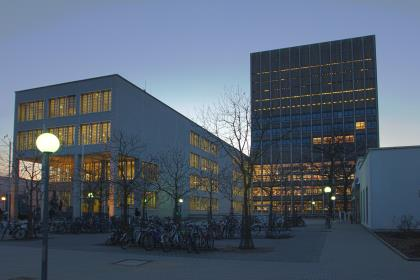
\includegraphics[width=\textwidth]{Abbildungen/bib.jpg}
	\caption{Außenansicht der KIT-Bibliothek. Bilder bitte immer manuell mit dem Parameter [h] setzen.	An dieser Stelle ist das Bild mit dem Figure-Parameter [h] platziert worden. Vor und nach der Figure-Umgebung steht eine Leerzeile.}
	\label{fig:bib}
\end{figure}

Lorem ipsum dolor sit amet, consetetur sadipscing elitr, sed diam nonumy eirmod tempor invidunt ut labore et dolore magna aliquyam erat, sed diam voluptua. At vero eos et accusam et justo duo dolores et ea rebum. Stet clita kasd gubergren, no sea takimata sanctus est Lorem ipsum dolor sit amet. Lorem ipsum dolor sit amet, consetetur sadipscing elitr, sed diam nonumy eirmod tempor invidunt ut labore et dolore magna aliquyam erat, sed diam voluptua. At vero eos et accusam et justo duo dolores et ea rebum. Stet clita kasd gubergren, no sea takimata sanctus est Lorem ipsum dolor sit amet. At vero eos et accusam et justo duo dolores et ea rebum.

Lorem ipsum dolor sit amet, consetetur sadipscing elitr, sed diam nonumy eirmod tempor invidunt ut labore et dolore magna aliquyam erat, sed diam voluptua. At vero eos et accusam et justo duo dolores et ea rebum. Stet clita kasd gubergren, no sea takimata sanctus est Lorem ipsum dolor sit amet. At vero eos et accusam et justo duo dolores et ea rebum.	

Lorem ipsum dolor sit amet, consetetur sadipscing elitr, sed diam nonumy eirmod tempor invidunt ut labore et dolore magna aliquyam erat, sed diam voluptua. At vero eos et accusam et justo duo dolores et ea rebum. Stet clita kasd gubergren, no sea takimata sanctus est Lorem ipsum dolor sit amet. At vero eos et accusam et justo duo dolores et ea rebum.

Curabitur a felis in nunc fringilla tristique. Morbi mattis ullamcorper velit. Phasellus gravida semper nisi. Nullam vel sem. Pellentesque libero tortor, tincidunt et, tincidunt eget, semper nec, quam. Sed hendrerit. Morbi ac felis. Nunc egestas, augue at pellentesque laoreet, felis eros vehicula leo, at malesuada velit leo quis pede. Donec interdum, metus et hendrerit aliquet, dolor diam sagittis ligula, eget egestas libero turpis vel mi. Nunc nulla. Fusce risus nisl, viverra et, tempor et.Pellentesque ut neque. Pellentesque habitant morbi tristique senectus et netus et malesuada fames ac turpis egestas. In dui magna, posuere eget, vestibulum et, tempor auctor, justo. 

%\newpage
\begin{figure}[h!] % "\begin{figure}" ist eine Umgebung für Gleitobjekte, damit die Abbildung nummeriert und beschriftet ("\caption{}")und mit einem Label ("\label{fig:bib}") versehen und darauf verwiesen werden kann ("\ref{fig:bib}")
	\centering
%\hspace{-7pt} % Horizontale verschiebung der Bildreihe
	\subfloat[Subfloat. Bild Nr. 1. Zweizeilige Bildunterschriften stehen im Flattersatz. Silbentrennung ist aktiviert.]{%
		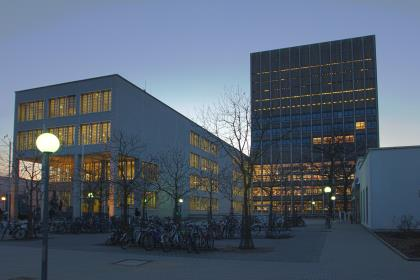
\includegraphics[width=0.49\linewidth]{Abbildungen/bib.jpg}%
	}
\hfill % Füllt den den vertikalen Abstand zwischen den Bildern auf, sofern die Bilder entsprechend klein sind
	\subfloat[Subfloat. Bild Nr. 2.]{%
		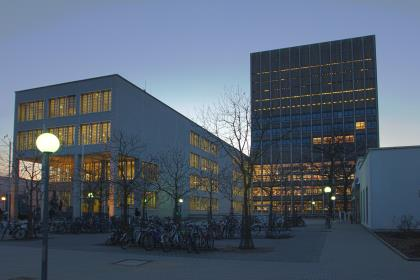
\includegraphics[width=0.49\linewidth]{Abbildungen/bib.jpg}%
	}
\\ \vspace{3mm} % Abstand zur zweiten Bildreihe % Plus Abstand aufgrund des Befehles "\captionsetup[subfloat]{belowskip=}" aus der Datei dokOptions.tex
%\hspace{-7pt} % Horizontale verschiebung der Bildreihe
	\subfloat[Subfloat. Bild Nr. 3. Das ist ein Beispiel für einen \linebreak manuellen Zeilenumbruch.]{%
		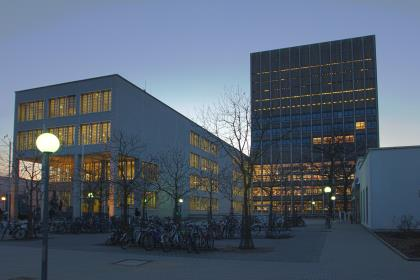
\includegraphics[width=0.49\linewidth]{Abbildungen/bib.jpg}%
	}
\hfill % Füllt den den vertikalen Abstand zwischen den Bildern auf, sofern die Bilder entsprechend klein sind
	\subfloat[Subfloat. Bild Nr. 4.]{%
		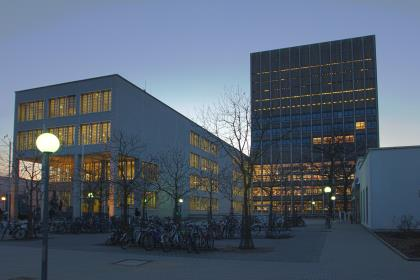
\includegraphics[width=0.49\linewidth]{Abbildungen/bib.jpg}%
	}
	\caption{Außenansicht der KIT-Bibliothek. Bilder bitte immer manuell mit dem Parameter [h] setzen.	An dieser Stelle ist das Bild mit dem Figure-Parameter [h] platziert worden. Vor und nach der Figure-Umgebung steht eine Leerzeile.}
	\label{fig:bib4}
\end{figure}

Aenean viverra rhoncus pede. Pellentesque habitant morbi tristique senectus et netus et malesuada fames ac turpis egestas. Ut non enim eleifend felis pretium feugiat vivamus quis mi. Phasellus a est. Phasellus magna. In hac habitasse platea dictumst. Curabitur at lacus ac velit ornare lobortis.\footnote{Cabo. Facerfe rferspient que nus molora doleserem. Ut a si autemo tectaquame enihil intota sam am ditati omnihil ma sequis re, aut fugiam earchil luptaque consequ.} Curabitur a felis in nunc fringilla tristique. Morbi mattis ullamcorper velit. Phasellus gravida semper nisi. Nullam vel sem. Pellentesque libero tortor, tincidunt et, tincidunt eget, semper nec, quam. Sed hendrerit.

%\newpage
Pellentesque habitant morbi tristique senectus et netus et malesuada fames ac turpis egestas. In dui magna, posuere eget, vestibulum et, tempor auctor, justo. In ac felis quis tortor malesuada pretium. Pellentesque auctor neque nec urna. Proin sapien ipsum, porta a, auctor quis, euismod ut, mi. Aenean viverra rhoncus pede. Pellentesque habitant morbi tristique senectus et netus et malesuada fames ac turpis egestas. Ut non enim eleifend felis pretium feugiat vivamus quis mi. Phasellus a est. Phasellus magna. In hac habitasse platea dictumst. Curabitur at lacus ac velit ornare lobortis. Aenean viverra rhoncus pede. Pellentesque habitant morbi tristique senectus et netus et malesuada fames ac turpis egestas. Ut non enim eleifend felis pretium feugiat vivamus quis mi. Phasellus a est. Phasellus magna. Phasellus a est. Phasellus magna. In hac habitasse platea dictumst. Curabitur at lacus ac velit ornare lobortis. Aenean viverra rhoncus pede. Pellentesque habitant morbi tristique senectus et netus et malesuada fames ac turpis egestas. Ut non enim eleifend felis pretium feugiat vivamus quis mi. Phasellus a est. Phasellus magna.

Phasellus magna. Phasellus a est. Phasellus magna. In hac habitasse platea dictumst. Curabitur at lacus ac velit ornare lobortis. Aenean viverra rhoncus pede. Pellentesque habitant morbi tristique senectus et netus et malesuada fames ac turpis egestas. Ut non enim eleifend felis pretium feugiat vivamus quis mi. 

%\newpage		 
\begin{figure}[h]
	\centering
	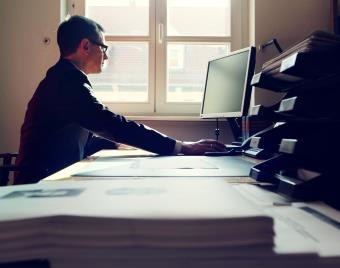
\includegraphics[width=6cm]{Abbildungen/wissen.jpg}
	\caption[Wissenschaftler an seinem Arbeitsplatz.]{Wissenschaftler an seinem Arbeitsplatz. Bilder bitte immer manuell mit dem Parameter [h] setzen. An dieser Stelle ist das Bild mit dem Figure-Parameter [h] platziert worden. Vor und nach der Figure-Umgebung steht eine Leerzeile.}
	\label{fig:wissen}
\end{figure}

Pellentesque habitant morbi tristique senectus et netus et malesuada fames ac turpis egestas. In dui magna, posuere eget, vestibulum et, tempor auctor, justo. In ac felis quis tortor malesuada pretium. Pellentesque auctor neque nec urna. Proin sapien ipsum, porta a, auctor quis, euismod ut, mi. Aenean viverra rhoncus pede. Pellentesque habitant morbi tristique senectus et netus et malesuada fames ac turpis egestas. Ut non enim eleifend felis pretium feugiat vivamus quis mi. Phasellus a est. Phasellus magna. In hac habitasse platea dictumst. Curabitur at lacus ac velit ornare lobortis.

Pellentesque habitant morbi tristique senectus et netus et malesuada fames ac turpis egestas. In dui magna, posuere eget, vestibulum et, tempor auctor, justo. In ac felis quis tortor malesuada pretium. Pellentesque auctor neque nec urna. Proin sapien ipsum, porta a, auctor quis, euismod ut, mi. Aenean viverra rhoncus pede. Pellentesque habitant morbi tristique senectus et netus et malesuada fames ac turpis egestas. Ut non enim eleifend felis pretium feugiat vivamus quis mi. Phasellus a est. Phasellus magna. In hac habitasse platea dictumst. Curabitur at lacus ac velit ornare lobortis. Pellentesque habitant morbi tristique senectus et netus et malesuada fames ac turpis egestas.

%Pellentesque habitant morbi tristique senectus et netus et malesuada fames ac turpis egestas. In dui magna, posuere eget, vestibulum et, tempor auctor. Pellentesque habitant morbi tristique senectus et netus et malesuada fames ac turpis egestas. In dui magna, posuere eget, vestibulum et, tempor auctor.

\begin{table}[h] % "\begin{table}" ist eine Umgebung für Gleitobjekte, damit die Tabelle "\begin{tabular}" nummeriert, übertitelt und mit einem Label versehen und darauf verwiesen werden kann
	\caption{Auch Tabellen (\glqq \textbackslash begin\{table\}\grqq{}) werden immer mit dem Parameter [h] eingefügt. Vor und nach der Tabellen-Umgebung steht eine Leerzeile.}
	\begin{tabularx}{\textwidth}{XXXXXXXX} \toprule
		Spalte1 & Spalte2 & Spalte3 & Spalte4 & Spalte5
		& Spalte6 & Spalte7 & Spalte8 \\ \midrule
		AA      & BB      & CC      & DD      &
		EE      & FF      & GG      & HH       \\
		AA      & BB      & CC      & DD
		& EE      & FF      & GG      & HH    \\
		AA      & BB      & CC      & DD
		& EE      & FF      & GG      & HH    \\
		AA      & BB      & CC      & DD
		& EE      & FF      & GG      & HH    \\
		AA      & BB      & CC      & DD
		& EE      & FF      & GG      & HH    \\
		AA      & BB      & CC      & DD
		& EE      & FF      & GG      & HH     \\ \bottomrule
	\end{tabularx}
\end{table}

Pellentesque habitant morbi tristique senectus et netus et malesuada fames ac turpis egestas. In dui magna, posuere eget, vestibulum et, tempor auctor. Pellentesque habitant morbi tristique senectus et netus et malesuada fames ac turpis egestas. In dui magna, posuere eget, vestibulum et, tempor auctor. In dui magna, posuere eget, vestibulum et, tempor auctor.

% Theorie
\markboth{Theorie}{Theorie}

\chapter{Theorie}
\label{cha:Theorie}
Lorem ipsum dolor sit amet, consetetur sadipscing elitr, sed diam nonumy eirmod tempor invidunt ut labore et dolore magna aliquyam erat, sed diam voluptua. At vero eos et accusam et justo duo dolores et ea rebum. Stet clita kasd gubergren, no sea takimata sanctus est Lorem ipsum dolor sit amet. Lorem ipsum dolor sit amet, consetetur sadipscing elitr, sed diam nonumy eirmod tempor invidunt ut labore et dolore magna aliquyam erat, sed diam voluptua. At vero eos et accusam et justo duo dolores et ea rebum. Stet clita kasd gubergren, no sea takimata sanctus est Lorem ipsum dolor sit amet.

Lorem ipsum dolor sit amet, consetetur sadipscing elitr, sed diam nonumy eirmod tempor invidunt ut labore et dolore magna aliquyam erat, sed diam voluptua. At vero eos et accusam et justo duo dolores et ea rebum. Stet clita kasd gubergren, no sea takimata sanctus est Lorem ipsum dolor sit amet. Lorem ipsum dolor sit amet, consetetur sadipscing elitr, sed diam nonumy eirmod tempor invidunt ut labore et dolore magna aliquyam erat, sed diam voluptua. At vero eos et accusam et justo duo dolores et ea rebum. Stet clita kasd gubergren, no sea takimata sanctus est Lorem ipsum dolor sit amet.

Lorem ipsum dolor sit amet, consetetur sadipscing elitr, sed diam nonumy eirmod tempor invidunt ut labore et dolore magna aliquyam erat, sed diam voluptua. At vero eos et accusam et justo duo dolores et ea rebum. Stet clita kasd gubergren, no sea takimata sanctus est Lorem ipsum dolor sit amet. Lorem ipsum dolor sit amet, consetetur sadipscing elitr, sed diam nonumy eirmod tempor invidunt ut labore et dolore magna aliquyam erat, sed diam voluptua. At vero eos et accusam et justo duo dolores et ea rebum. Stet clita kasd gubergren, no sea takimata sanctus est Lorem ipsum dolor sit amet.

\begin{table}[h] % "\begin{table}" ist eine Umgebung für Gleitobjekte, damit die Tabelle "\begin{tabular}" nummeriert, übertitelt und mit einem Label versehen und darauf verwiesen werden kann
	\caption[Od quo tecto offic torit eteum acerum fuga. Ideni omnihic idundero doluptus iminvel luptati busdaepta sequi dolorec tatessinum.]{Auch Tabellen (\glqq \textbackslash begin\{table\}\grqq{}) werden immer mit dem Parameter [h] eingefügt. Vor und nach der Tabellen-Umgebung steht eine Leerzeile. Fügen sie mit \glqq \textbackslash newline\grqq{} manuelle Zeilenumbrüche ein, wenn die Abstände zwischen den Wörtern in einer Zelle zu groß werden.}
	\centering
	\begin{tabular}{ | l | l | l | p{2.5cm} |}
			\hline
			Aliquyam & Dolor & Rebum & Sadipscing \\ \hline
			Invidunt & Labore & Sanctus & Stet clita kasd \newline gubergren. \\ \hline
			Magna & Gubergren & Clita & No sea takimata \newline sanctus. \\ \hline
			Eirmod & Voluptua & Aliquyam & Sed diam nonumy eirmod tempor. \\
			\hline%
	\end{tabular}%
	\label{tab:tab}%
\end{table}%

Od quo tecto offic torit eteum acerum fuga. Ideni omnihic idundero doluptus iminvel luptati busdaepta sequi dolorec tatessinum quas et quia perae et qui blanditi quiberit alique provit, cus incipid ut quis enis vel id es asperum volor aut unt, quatum eturem aciassin et rest inulluptam et volecae. Od quo tecto offic torit eteum acerum fuga. Ideni omnihic idundero doluptus iminvel luptati busdaepta sequi dolorec tatessinum quas et quia perae et qui blanditi quiberit alique provit, cus incipid ut quis enis vel id es asperum volor aut unt, quatum eturem aciassin et rest inulluptam et volecae. Od quo tecto offic torit eteum acerum fuga. Ideni omnihic idundero doluptus iminvel luptati busdaepta sequi dolorec tatessinum quas et quia perae et qui blanditi quiberit alique provit, cus incipid ut quis enis vel id es asperum volor aut unt, quatum eturem aciassin et rest inulluptam et volecae. Od quo tecto offic torit eteum acerum fuga. Ideni omnihic idundero doluptus iminvel luptati busdaepta sequi dolorec tatessinum quas et quia perae et qui blanditi quiberit alique provit, cus incipid ut quis enis vel id es asperum volor aut unt, quatum eturem aciassin et rest inulluptam et volecae.
\begin{subequations}
	\label{maxwell-gleichungen}
	\begin{align}
	\text{div }(\vec{D}) &= 4 \cdot \pi \cdot \rho
	\label{coulomb-gesetz}\\
	\text{rot }(\vec{H}) &= \frac{4 \cdot \pi}{c} \cdot \vec{j}
	\label{ampere-gesetz}\\
	\text{rot }(\vec{E}) &= - \frac{1}{c} \cdot \frac{\partial \vec{B}}{\partial t}
	\label{faraday-gesetz-1} \\
	\text{div }(\vec{B}) &= 0
	\label{faraday-gesetz-2}
	\end{align}
\end{subequations}
Arepelisti re denda doluptata quo demque conseribeate eum quiberor aut quatur maiorae riberis eserio eaturepro ommo bero eum que quisquidit volendis eni asi sint aut pe minis is re nonseque ius aut pa is expel ium nobis miliquati dolupit, qui nullanis re, sitiis si volor mo te eventia vendit qui dolupta quamusda vereped magnihi cturem dendignatus vite prernatatis soluptat aperum sequostorum et quistru pienitiis arum, optaquo qui comnis cuptam qui officitate pellent ariae occaborrovid mod esequi dolorum rerro quas vent harciistia quis voloris sinctiis ea nistrum facius simus utem sit, inctor sit dolorrum ditio. Ecerum et est quia doluptur? Qui dolorero des nosapis exerias dest, qui coratur itemporum repeliq uiassit, inum fugiasi simil est alicium ilis que nimusanis es suntiaestrum ium ium harcil iligent excearum fugia nonsequia dem.
% Binomialkoeffizient:
\begin{align*}
\binom{n}{k} = \frac{n!}{(n - k)! \cdot k!}
\end{align*}
Optaquo qui comnis cuptam qui officitate pellent ariae occaborrovid mod esequi dolorum rerro quas vent harciistia quis voloris sinctiis ea nistrum facius simus utem sit, inctor sit dolorrum ditio. Ecerum et est quia doluptur? Qui dolorero des nosapis exerias dest, qui coratur itemporum repeliq uiassit, inum fugiasi simil est alicium ilis que nimusanis es suntiaestrum ium ium harcil iligent excearum fugia nonsequia dem.
\begin{equation} 
\prod \limits_{i=1}^{n+1}i = 1\cdot 2\cdot\dots\cdot n\cdot (n+1) \
\end{equation}
Arepelisti re denda doluptata quo demque conseribeate eum quiberor aut quatur maiorae riberis eserio eaturepro ommo bero eum que quisquidit volendis eni asi sint aut pe minis is re nonseque ius aut pa is expel ium nobis miliquati dolupit, qui nullanis re, sitiis si volor mo te eventia vendit qui dolupta quamusda vereped magnihi cturem dendignatus vite prernatatis soluptat aperum sequostorum et quistru pienitiis arum, optaquo qui comnis cuptam qui officitate pellent ariae occaborrovid mod esequi dolorum rerro quas vent harciistia quis voloris sinctiis ea nistrum facius simus utem sit, inctor sit dolorrum ditio. Ecerum et est quia doluptur? Qui dolorero des nosapis exerias dest, qui coratur itemporum repeliq uiassit, inum fugiasi simil est alicium ilis que nimusanis es suntiaestrum ium ium harcil iligent excearum fugia nonsequia dem. Ovidus.

% Überschriften
% \chapter{Überschriften}

% Stehen zwei Überschriften direkt untereinander, muss die Autorin oder der Autor zwischen den Überschriften manuell eine Anpassung des vertikalen Abstands mit dem Befehl \glqq vspace\grqq{} vornehmen. Für die folgende Aneinanderreihung der Überschriften entnehmen Sie den vertikalen Abstand bitte wie folgt:

% \begin{itemize}

% \item \raggedright Zwischen \glqq chapter\grqq{} und \glqq section\grqq{} bitte mit dem Befehl \glqq vspace\grqq{} einen zusätzlichen vertikalen Abstand einfügen von \hbox{-}3~mm. 
% \begin{Verbatim}
% \chapter{Überschrift Ebene Chapter}
% \vspace{-3mm}
% \section{Überschrift Ebene Section}
% \end{Verbatim}
% (Sollabstand: 10~mm, gemessen von der Grundlinie der Überschrift \glqq chapter\grqq{} zur H-Linie der Überschrift \glqq section\grqq{}) 

% \item \raggedright Zwischen \glqq section\grqq{} und \glqq subsection\grqq{} bitte mit dem Befehl \glqq vspace\grqq{} einen zusätzlichen vertikalen Abstand einfügen von 2~mm. 
% \begin{Verbatim}
% \section{Überschrift Ebene Section}
% \vspace{2mm}
% \subsection{Überschrift Ebene Subsection}
% \end{Verbatim}
% (Sollabstand: 10~mm, gemessen von der Grundlinie der Überschrift \glqq section\grqq{} zur H-Linie der Überschrift \glqq subsection\grqq{})

% \item \raggedright Zwischen \glqq subsection\grqq{} und \glqq subsubsection\grqq{} bitte mit dem Befehl \glqq vspace\grqq{} einen zusätzlichen vertikalen Abstand einfügen von 3~mm. 
% \begin{Verbatim}
% \subsection{Überschrift Ebene Subsection}
% \vspace{3mm}
% \subsubsection{Überschrift Ebene Subsubsection}
% \end{Verbatim}
% (Sollabstand: 10~mm, gemessen von der Grundlinie der Überschrift \glqq subsection\grqq{} zur H-Linie der Überschrift \glqq subsubsection\grqq{}. 

% \end{itemize}

% % Für die exakte Angabe des Befehls \glqq vspace\grqq{} mit den entsprechenden Werten sehen Sie bitte in die Datei \glqq content\_vorlage/ueberschriften.tex\grqq{}. 
% Das Ergebnis mit den entsprechenden vertikalen Abständen zwischen den Überschriften sehen Sie in Kapitel \ref{chap:UeberschriftenEbenen} (\glqq \nameref{chap:UeberschriftenEbenen}\grqq{}) auf Seite \pageref{chap:UeberschriftenEbenen} in dieser PDF-Datei.



\chapter{Überschrift Ebene 1 (chapter)}
\label{chap:UeberschriftenEbenen}
% Lorem ipsum dolor sit amet, consectetuer adipiscing elit. Aenean co~mmodo ligula eget dolor. Aenean massa.
% \vspace{-3mm} % Folgt kein Text nach der Überschrift, muss der Abstand zur nächsten Überschrift manuell angepasst werden

\section{Überschrift Ebene 2 (section)}
% Lorem ipsum dolor sit amet, consectetuer adipiscing elit. Aenean co~mmodo ligula eget dolor. Aenean massa.
\vspace{1.5mm} % Folgt kein Text nach der Überschrift, muss der Abstand zur nächsten Überschrift manuell angepasst werden 

\subsection{Überschrift Ebene 3 (subsection)}
% Lorem ipsum dolor sit amet, consectetuer adipiscing elit. Aenean co~mmodo ligula eget dolor. Aenean massa.
\vspace{3mm} % Folgt kein Text nach der Überschrift, muss der Abstand zur nächsten Überschrift manuell angepasst werden

\subsubsection{Überschrift Ebene 4 (subsubsection)}
% Lorem ipsum dolor sit amet, consectetuer adipiscing elit. Aenean co~mmodo ligula eget dolor. Aenean massa.


% Zusammenfassung und Ausblick
\markboth{Zusammenfassung und Ausblick}{Zusammenfassung und Ausblick}
\chapter{Zusammenfassung und Ausblick}
\label{cha:Zusammenfassung und Ausblick}

%%%%%%%%%%%%%%%%%%%%%%%%%%%%%%%%%%%%%%%%%%%%%%%%%%

\section{Zusammenfassung}
\label{sec:Zusammenfassung}
Arepelisti re denda doluptata quo demque conseribeate eum quiberor aut quatur maiorae riberis eserio eaturepro ommo bero eum que quisquidit volendis eni asi sint aut pe minis is re nonseque ius aut pa is expel ium nobis miliquati dolupit, qui nullanis re, sitiis si volor mo te eventia vendit qui dolupta quamusda vereped magnihi cturem dendignatus vite prernatatis soluptat aperum sequostorum et quistru pienitiis arum, optaquo qui comnis cuptam qui officitate pellent ariae occaborrovid mod esequi dolorum rerro quas vent harciistia quis voloris sinctiis ea nistrum facius simus utem sit, inctor sit dolorrum ditio. Ecerum et est quia doluptur? Qui dolorero des nosapis exerias dest, qui coratur itemporum repeliq uiassit, inum fugiasi simil est alicium ilis que nimusanis es suntiaestrum ium ium harcil iligent excearum fugia nonsequia dem.

Arepelisti re denda doluptata quo demque conseribeate eum quiberor aut quatur maiorae riberis eserio eaturepro ommo bero eum que quisquidit volendis eni asi sint aut pe minis is re nonseque ius aut pa is expel ium nobis miliquati dolupit, qui nullanis re, sitiis si volor mo te eventia vendit qui dolupta quamusda vereped magnihi cturem dendignatus vite prernatatis soluptat aperum sequostorum et quistru pienitiis arum, optaquo qui comnis cuptam qui officitate pellent ariae occaborrovid mod esequi dolorum rerro quas vent harciistia quis voloris sinctiis ea nistrum facius simus utem sit, inctor sit dolorrum ditio. Ecerum et est quia doluptur? Qui dolorero des nosapis exerias dest, qui coratur itemporum repeliq uiassit, inum fugiasi simil est alicium ilis que nimusanis es suntiaestrum ium ium harcil iligent excearum fugia nonsequia dem.

\section{Ausblick}
\label{sec:Ausblick}
Arepelisti re denda doluptata quo demque conseribeate eum quiberor aut quatur maiorae riberis eserio eaturepro ommo bero eum que quisquidit volendis eni asi sint aut pe minis is re nonseque ius aut pa is expel ium nobis miliquati dolupit, qui nullanis re, sitiis si volor mo te eventia vendit qui dolupta quamusda vereped magnihi cturem dendignatus vite prernatatis soluptat aperum sequostorum et quistru pienitiis arum, optaquo qui comnis cuptam qui officitate pellent ariae occaborrovid mod esequi dolorum rerro quas vent harciistia quis voloris sinctiis ea nistrum facius simus utem sit, inctor sit dolorrum ditio. Ecerum et est quia doluptur? Qui dolorero des nosapis exerias dest, qui coratur itemporum repeliq uiassit, inum fugiasi simil est alicium ilis que nimusanis es suntiaestrum ium ium harcil iligent excearum fugia nonsequia dem.



% Schlussfolgerungen und Ausblick
%\include{Inhalt/07_Schlussfolgerungen_und_Ausblick}

%%%%%%%%%%%%%%%%%%%%%%%%%%%%%%%%%%%%%%%%%%%%%%%%%%
%%%				Anhang! (include)	 		               %%%
%%%%%%%%%%%%%%%%%%%%%%%%%%%%%%%%%%%%%%%%%%%%%%%%%%

% Anhang; Kapitel im Anhang erhalten Großbuchstaben im Inhaltsverzeichnis
\appendix 

\markboth{Anhang}{Anhang}
\chapter{Anhang}
\label{cha:Anhang}

%%%%%%%%%%%%%%%%%%%%%%%%%%%%%%%%%%%%%%%%%%%%%%%%%%

Lorem ipsum dolor sit amet, consetetur sadipscing elitr, sed diam nonumy eirmod tempor invidunt ut labore et dolore magna aliquyam erat, sed diam voluptua. At vero eos et accusam et justo duo dolores et ea rebum. Stet clita kasd gubergren, no sea takimata sanctus est Lorem ipsum dolor sit amet. Lorem ipsum dolor sit amet, consetetur sadipscing elitr, sed diam nonumy eirmod tempor invidunt ut labore et dolore magna aliquyam erat, sed diam voluptua. At vero eos et accusam et justo duo dolores et ea rebum. Stet clita kasd gubergren, no sea takimata sanctus est Lorem ipsum dolor sit amet.

%%%%%%%%%%%%%%%%%%%%%%%%%%%%%%%%%%%%%%%%%%%%%%%%%%
%%%				Verzeichnisse! (include)	           %%%
%%%%%%%%%%%%%%%%%%%%%%%%%%%%%%%%%%%%%%%%%%%%%%%%%%

% Abbildungsverzeichnis! lof! listoffigures!
\renewcommand{\listfigurename}{Abbildungsverzeichnis} % Ändert die Überschrift und das Lesezeichen in der PDF-Datei von "List of Figures" in "Tabellenverzeichnis"; dieser Befehl ist lokalitätsgebunden
\listoffigures
% \addcontentsline{toc}{chapter}{\listfigurename} % Aufgrund des in der Dokumentklasse "book" angegebenen optionalen Parameters "listof=totoc" ist diese Befehlszeile nicht nötig

% Tabellenverzeichnis! lot! listoftables!
\renewcommand{\listtablename}{Tabellenverzeichnis} % Ändert die Überschrift und das Lesezeichen in der PDF-Datei von "List of Tables" in "Tabellenverzeichnis"; dieser Befehl ist lokalitätsgebunden
\listoftables
% \addcontentsline{toc}{chapter}{\listtablename} % Aufgrund des in der Dokumentklasse "book" angegebenen optionalen Parameters "listof=totoc" ist diese Befehlszeile nicht nötig

% Listingsverzeichnis! listoflistings! 
% \renewcommand{\lstlistlistingname}{Listingsverzeichnis} % Ändert die Überschrift und das Lesezeichen in der PDF-Datei von "List " in "Listingsverzeichnis"; diese Befehl ist lokalitätsgebunden
\renewcommand{\lstlistlistingname}{\latex-Quellcode-Verzeichnis} % Ändert die Überschrift und das Lesezeichen in der PDF-Datei von "List " in "Listingsverzeichnis"; diese Befehl ist lokalitätsgebunden
% \lstlistoflistings

% Literaturverzeichnis!
\markboth{Literaturverzeichnis}{Literaturverzeichnis}

%%%%%%%%%%%%%%%%%%%%%%%%%%%%%%%%%%%%%%%%%%%%%%%%%%

\chapter*{Eigene Veröffentlichungen}
\addcontentsline{toc}{chapter}{Eigene Veröffentlichungen}

\section*{Journalartikel}
\addcontentsline{toc}{section}{Journalartikel}
\renewcommand{\refnamejournal}{Journalartikel}
\begingroup % Überschrift von \bibliography{} löschen
\renewcommand{\chapter}[2]{}
\renewcommand{\section}[2]{}
\nocitejournal{*} % Alle Titel der .bib-Datei im Literaturverzeichnis anzeigen, wenn aktiviert; bei Deaktivierung werden nur die zitierten Titel angezeigt
\bibliographystylejournal{plainnat} % Zitierstil bei Bedarf anpassen
\bibliographyjournal{Literatur/Eigene_Journal_Papers}{}
\endgroup

%%%%%%%%%%%%%%%%%%%%%%%%%%%%%%%%%%%%%%%%%%%%%%%%%%

\section*{Konferenzbeitr\"age}
\addcontentsline{toc}{section}{Konferenzbeiträge}
\renewcommand{\refnameconference}{Konferenzbeiträge}
\begingroup % Überschrift von \bibliography{} löschen
\renewcommand{\chapter}[2]{}
\renewcommand{\section}[2]{}
\nociteconference{*} % Alle Titel der .bib-Datei im Literaturverzeichnis anzeigen, wenn aktiviert; bei Deaktivierung werden nur die zitierten Titel angezeigt
\bibliographystyleconference{plainnat} % Zitierstil bei Bedarf anpassen
\bibliographyconference{Literatur/Eigene_Konferenz_Papers}{}
\endgroup

%%%%%%%%%%%%%%%%%%%%%%%%%%%%%%%%%%%%%%%%%%%%%%%%%%

\chapter*{Literaturverzeichnis}
\addcontentsline{toc}{chapter}{Literaturverzeichnis}
\renewcommand{\refname}{Literaturverzeichnis}
\renewcommand\bibname{Literaturverzeichnis}
\begingroup % Überschrift von \bibliography{} löschen
\renewcommand{\chapter}[2]{}
\renewcommand{\section}[2]{}
\nocite{*} % Alle Titel der .bib-Datei im Literaturverzeichnis anzeigen, wenn aktiviert; bei Deaktivierung werden nur die zitierten Titel angezeigt
\bibliographystyle{plainnat} % Zitierstil bei Bedarf anpassen
\bibliography{Literatur/Externe_Literatur}{}
\endgroup

%%%%%%%%%%%%%%%%%%%%%%%%%%%%%%%%%%%%%%%%%%%%%%%%%%

%\markboth{Literaturverzeichnis}{Literaturverzeichnis}
%\renewcommand{\refname}{Literaturverzeichnis}
%\renewcommand\bibname{Literaturverzeichnis}
%\bibliography{Literatur/Eigene_Konferenz_Papers}{}
%\bibliographystyle{alpha}
%\nocite{*}

\end{document}